\documentclass[12pt]{UoAthesis} 
\usepackage{booktabs} 
\usepackage{color}
\usepackage{graphics}
\usepackage{enumerate}
\thesistitle{Honours Dissertation}
\thesisauthor{Christopher James Thomson} 
\thesispdfkeywords{}
\thesisyear{2012}

\thesisabstract{The objective of this thesis is to determine a general
  technique for converting continuous potentials to equilivant discrete
  potentials. Discrete potentials have many desirable properties. 
}

\acknowledgements{I would like to dedicate this work to..}

%%% The bibtex file where your references are stored 
\bibliography{main}
\begin{document}

%%% = = = DISSERTATION OVERVIEW = = =

% - INTRODUCTION - %
% Molecules, why are we interested in the molecular scale? What processes are molecular
% - - Molecular dynamics, what is it, why is it important to Chemical
%engineering.

% - - Leading into potentials, need for faster methods, more accurate methods.%
%Review of exisiting literature (Chapela, PRIME SPEADMD), what they've done,
%why its not as good as what you're going to do % 

% Outline of the thesis to come

% - Molecular Simulation 
% -- Newtonian mechanics F=MA, is it valid? 
% -- Forces from potentials (conservative forces) 
% Types of forces (gravitional (which is neglected)), pairwise forces 
% leading to intermolecular potentials.

% --- Give an example soft potential (LJ), Introduce a discrete -- 
% -potential,hard sphere is the prototypical discrete potential, -- 
% -but there are steppedpotentials too (Chapela). Talk about the -- 
% -advantages/disadvantages etc.

%%%% Lead out of the chapter with this 
% --- Introduce discrete potentials, say they need a special method of solution
%(EDMD).
% - Simulation Methods - % 
% - -Force Driven Simulators 
% - - - Introduction and general algorithm 
% - - -Integrators: Euler, Verlet, Velocity Verlet, Gear...lit review to find
%more recent ones
% - - - Optimization: neighbour lists, truncation of the potential 
%- - - Adv/Disadv? or just within other relevant topics 
% - - Event Driven Simulators % - - - Introduction and general algorithm 
% - - - Collision rules 
%Actually older than force based, although not as popular.
% - - - Optimization: neighbour lists, O(1) priority queue algorithms, time warp%algorithms
% - -Measuring System Properties % - - - Radial Distribution Function
 % - - -Temperature 
% - - - Pressure 
% - - - Coefficient of Diffusion 
% - Results - % 
 % - Discussion- % 
% - Conclusions - % 
% - Recommendations for future work - % 
% - Appendices -% 
% - - Derivation of collision rule for stepped potentials %
%% = = = END OVERVIEW = = = %%%

\chapter{Introduction}

Process simulation packages have become an integral part of chemical
engineering design. Central to these simulation software packages is
the ability to calculate thermodynamic and transport properties of
fluids quickly and accurately. Many modern processes rely on molecular
scale effects... (Absorption, membrane technology (reverse osmosis),
catalysis)....

\nomenclature[A]{MD}{Molecular Dynamics}

To better understand these large scale systems, we need to improve our
understanding of the smaller scales. Experiments are hard, can't hold
a ruler up to a molecule, everything is too fast, too small to
see. (X-ray crystallography). theory is hard, lots of molecules, can't
solve even three molecules motion analytically (need
cite). simulations are great, don't try to solve analytically. Since
50's (alder wainwright), computers are faster, modern sims are
amazing.

At the heart of these simulations are models for the atoms and
molecules involved. There are two classes of models, discrete and
contiuous.

%paragraph describing the thesis
In chapter~\ref{chap:one}, the something is discussed

\chapter{Molecular Models}
In this chapter, the dynamics and models used to represent molecular
systems are discussed. First, the arguments for selecting classical
mechanics over quantum mechanics as the underlying dynamics for the
simulations are presented.  Then, the two major classifications of the
available classical models, discrete and continuous potentials, are
discussed.

\section{Classical Mechanics}

\subsection{Validity of Classical Mechanics}

The underlying assumption behind many molecular dynamics simulations
is that the particles move according to the laws of classical
mechanics. Strictly, atoms and molecules should be treated using
quantum mechanics, due to their size and speed.  However molecular
dynamics makes two assumptions that allow these quantum mechanical
effects to be ignored.

The first is the Born-Oppenheimer Approximation which allows the
motion of electrons and the nucleus to be treated separately.  Since
the nucleus is much larger than the electrons and hence less affected
by quantum mechanics, it is treated as a classical particle.  The
electrons on the other hand are represented using a
potential~\cite{Jasper2006}.

The second assumption is that any quantum mechanical effects should
average out. Molecular dynamics is rarely interested in the motion of
a single electron, it is more concerned with the statistical average
over every particle.

These assumtions are usually valid unless very light atoms (such as
hydrogen or helium) are being simulated, or the particles are vibrating
at very high rates~\cite{Frenkel2002}.

\subsection{Newton's Second Law of Motion \label{NewtonLaw}}

The fundamental identity of classical mechnanics is Newton's Second
Law of Motion (Eq.~\eqref{eq:Fma}). This equation allows the
prediction of a particle's trajectory provided that an initial
position and velocity is known; and the forces acting on that particle
can be calculated for any position or velocity.

\begin{equation}
  \mathbf{F} = m\mathbf{a}
  \label{eq:Fma} 
\end{equation}
\nomenclature[V]{$F$}{Force}%
\nomenclature[V]{$m$}{Mass of a particle $i$}%
\nomenclature[V]{$\mathbf{a}$}{Acceleration vector of a particle}%

If a force depends only on the position of a particle, it is known as a
conservative force. Almost all forces considered in molecular dynamics
are of this type because atoms or molecules do not lose energy due to
friction or any other dissipative process.

Conservative molecular forces can be of one of two types.  The first
are body forces, which only depend on a single particle's absolute
position, such as gravity.  However gravity is usually disregarded in
MD as atoms and molecules have such low masses that gravity has very
little effect on them.

The second and most important type are intermolecular forces that
depend on position relative to other particles. In general, the
intermolecular forces are a function of all particle positions;
However, usually the total force acting on a particle $i$ is assumed
to be a sum of the forces between $i$ and every other particle
$j$. This is known as the binary interaction assumption and the
summation of forces is given by
\begin{equation}
  \mathbf{F}_i = \sum_{j \not= i}^{N}\mathbf{F}_{ij}
  \label{eq:pairwise}
\end{equation}
\nomenclature[V]{$F_{i}$}{Force acting on particle $i$}%
\nomenclature[V]{$F_{ij}$}{Intermolecular force between particle $i$
  and $j$}%
where $N$ is the total number of particles in the system.  Force
calculations are limited to pairs as this is simpler, but there are
examples of n-body forces available in the literature (e.g.\ see
Ref.~\cite{Tersoff1988}).

%Here the force between particles $i$ and $j$ is
%split into a repulsive force ($\mathbf{F}_R$) and an attractive force
%($\mathbf{F}_A$).  The coefficient in front of the repulsive force,
%$a$, is a range limiting term, while the coefficient $b$, is the bond
%order.  This describes the environment the particles are in, and
%strengthens or weakens the attractive force appropriately.
%
%\begin{equation}
%  \mathbf{F}_{ij} = a\mathbf{F}_{R} + b\mathbf{F}_A
%  \label{eq:tersoff}
%\end{equation}

The intermolecular forces used in molecular dynamics are frequently
described using a potential.  Provided that the force is conservative,
it can be calculated from its potential using the following equation
\begin{equation} 
  \mathbf{F}_{ij}=-\nabla \Phi_{ij}
  \label{eq:forcePotential} 
\end{equation}
\nomenclature[V]{$\Phi_{ij}$}{Intermolecular potential between
  particles $i$ and $j$}%
\nomenclature[O]{$\nabla$}{Gradient operator}%
where $\nabla$ denotes the gradient of the potential,
$\Phi_{ij}$. Using this definition, it is clear to see that by
defining an intermolecular potential, the intermolecular forces are
also described.  In the literature, intermolecular force fields are
usually described using potentials and in the following sections the
two types of potentials will be discussed.

\section{Continuous Potentials}
Models for the intermolecular interactions are typically defined using
functions for the potential energies between molecules.  A very
popular potential used in molecular dynamics simulations is the
Lennard-Jones potential \cite{Lennard-Jones1924} given by the
following expression
\begin{equation} 
  \Phi(r) = 4 \varepsilon \left[ \left( \frac{\sigma}{r} \right)^{12}
    -\left( \frac{\sigma}{r} \right)^{6} \right] 
  \label{eq:LJ} 
\end{equation}
\nomenclature[V]{$\varepsilon$}{Characteristic energy, usually well
  depth}%
\nomenclature[V]{$\sigma$}{Characteristic length, taken to be particle
  diameter}%
where $\varepsilon$ is the depth of the energy well and $\sigma$ is
the distance where the potential between two particles is zero. This
is illustrated in Fig.~\ref{fig:ljPot}. Despite its simplicity, it
gives comparable results to experimental values \cite{Rahman1964} for
noble gases due to their monatomic nature.

\begin{figure}[htp] 
  \begin{center}
    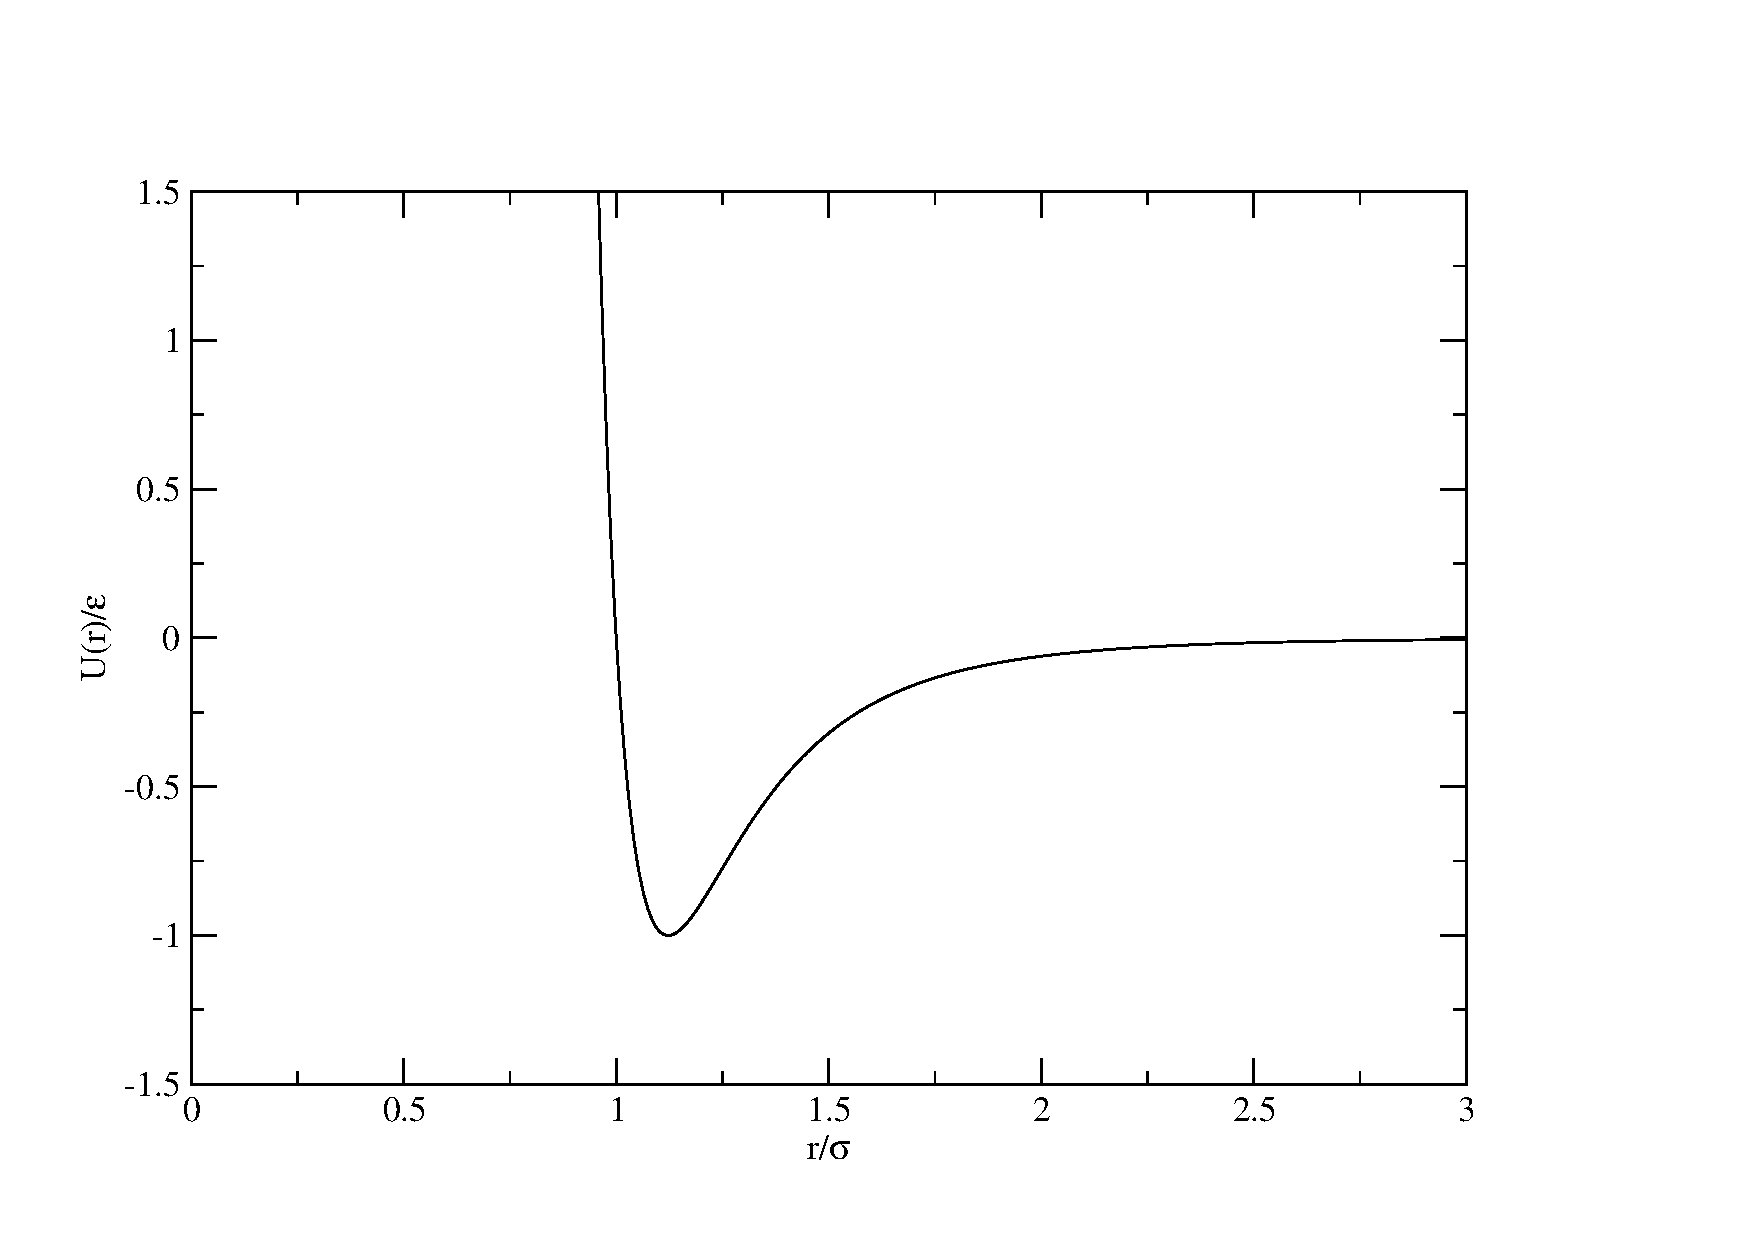
\includegraphics[clip,width=\textwidth]{figures/ljPlot} 
    \caption{\label{fig:ljPot} Plot of the Lennard-Jones potential}
  \end{center}
\end{figure}

The power 12 term, $\left(\sigma/r\right)^{12}$, gives the potential a
repulsive core caused by Pauli repulsion of overlapping electron
shells.  This repulsion is more accurately represented by an
exponential function which forms the basis of the Buckingham potential
\cite{Buckingham1938}.  However the Buckingham potential is not as
popular as the Lennard-Jones potential because the expontential
function is more computationally expensive to
calculate~\cite{White1997}.

The power 6 term, $\left(\sigma/r\right)^{6}$, in the Lennard-Jones
potential represents the attractive Van der Waals forces.  This
attractive well and repulsive core can be seen in the force plot 
of the Lennard-Jones potential, Fig.~\ref{fig:ljForce}.

\begin{figure}[htp] 
  \begin{center}
    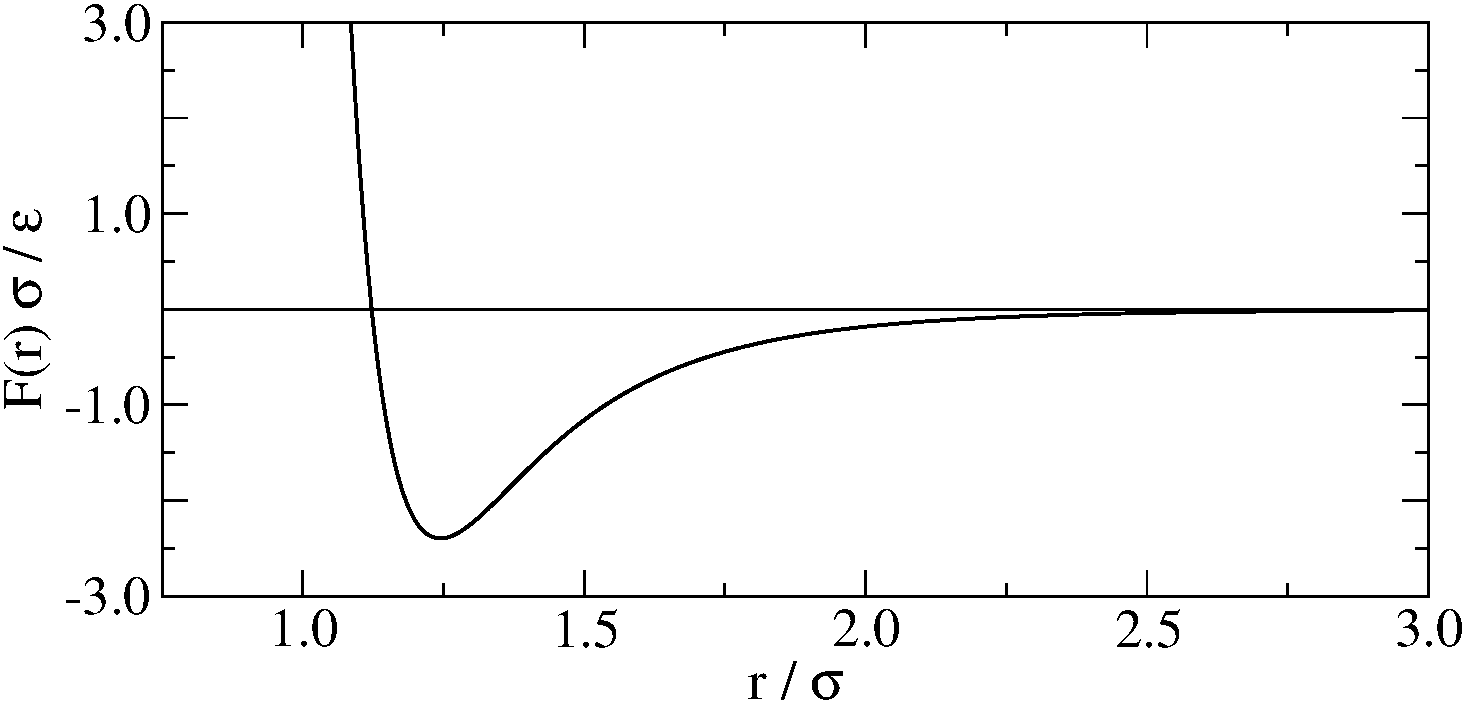
\includegraphics[clip,width=\textwidth]{figures/ljForce} 
    \caption{\label{fig:ljForce} Plot of the force between
      a pair of Lennard-Jones particles separated by a distance $r$}
  \end{center}
\end{figure}
\begin{align}
  \label{eq:CHARMMPotential}
  \Phi &= \sum_{\text{bonds}}k_b(r-r_0)^2  
  + \sum_{UB}K_{UB}(S-S_0)^2 
  + \sum_{\text{angles}}k_\theta(\theta - \theta_0)^2 \nonumber\\
  &+ \sum_{\text{dihedrals}} k_\chi[1+\cos(n\chi - \delta)] 
  + \sum_{\text{improper}} k_\psi(\psi - \psi_0)^2 \nonumber\\
  &+ \sum_{i=1}^{N-1}\sum_{j>i}^{N}\left\{ 4 \varepsilon 
    \left[ \left( \frac{\sigma}{r_{ij}} \right)^{12}
      -\left( \frac{\sigma}{r_{ij}} \right)^{6} \right] 
    + \frac{q_iq_j}{r_{ij}}\right\}
\end{align}
The Lennard-Jones potential can be included in part of more complex
potentials such as the CHARMM (Chemistry at HARvard Molecular
Mechanics) potential for simulating proteins
(Eq.~\eqref{eq:CHARMMPotential})~\cite{MacKerell1998}.  Here the
Lennard-Jones potential is used to represent Van der Waals forces
while Coulomb's Law $\left(\frac{q_iq_j}{r_{ij}}\right)$ is modelling
longer range electrostatic interactions.  The first five terms of
Eq.~\eqref{eq:CHARMMPotential} are contraints on bond movements
(streching, Urey-Bradley bond vibration, angle bending, dihedral
angle, and improper dihedral angle motion respectively, see
Ref.~\cite{Spoel2010} for descriptions of these bond movements).


\section{Discrete Potentials}

Discrete potentials differ from continuous potentials because they
have discontinuities.  The simplest discrete potential is that of the
hard sphere (see Fig.~\ref{fig:hardSphere}).

\begin{figure}[htp] 
  \begin{center}
    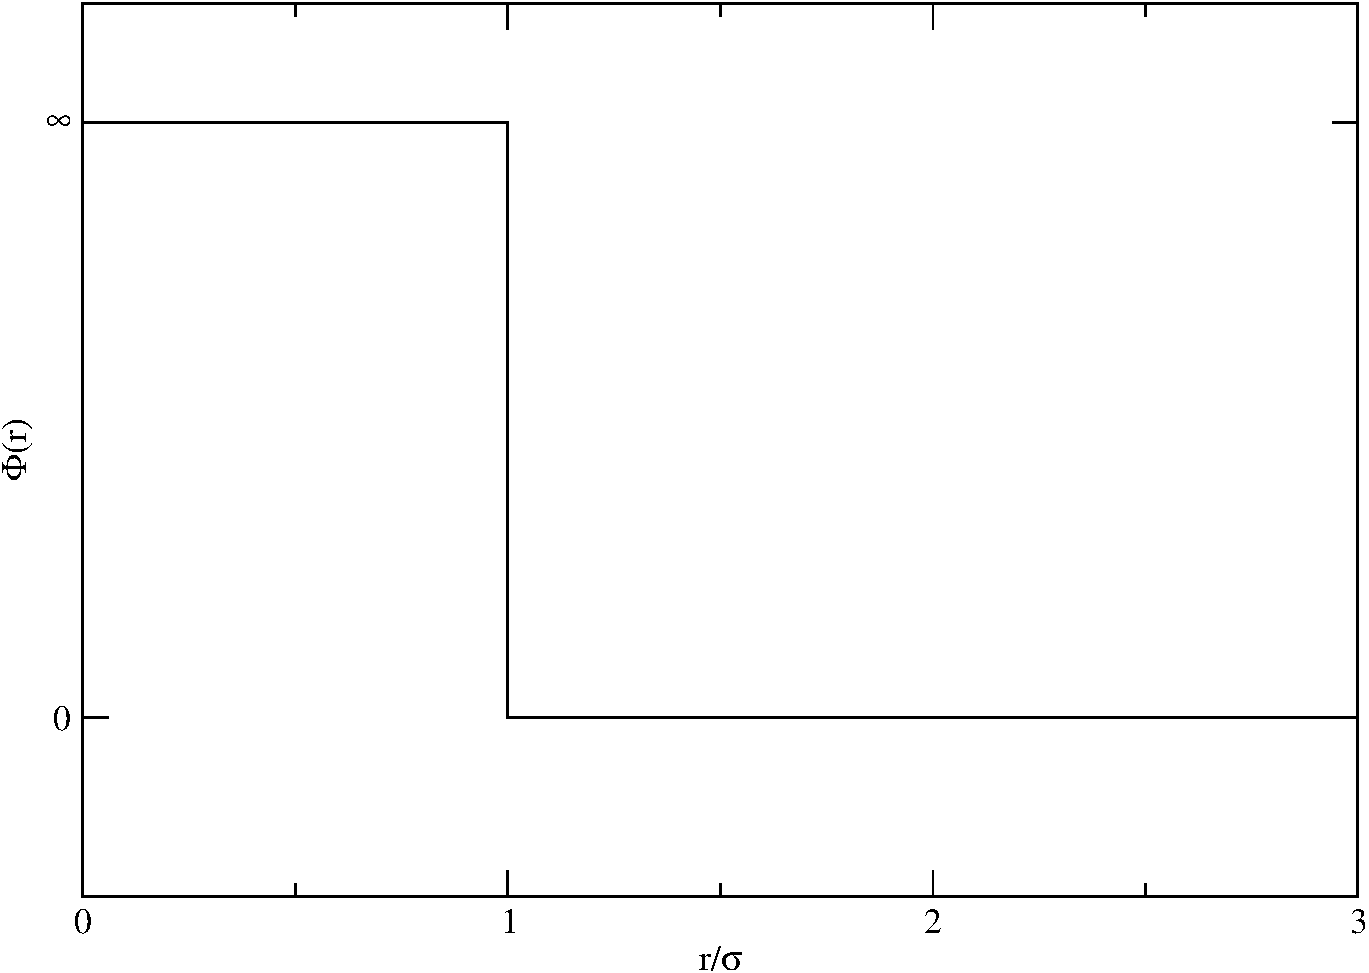
\includegraphics[clip,scale = 0.45]{figures/hardSphere} 
    \caption{\label{fig:hardSphere} Plot of the hard sphere potential}
  \end{center}
\end{figure}

Hard spheres were the first molecular models ever simulated
\cite{Alder1957} due to their relative simplicity.  The potential for
hard spheres is shown in equation \eqref{eq:potentialHS}, where
$\sigma$ is the diameter of the spheres.

\begin{equation}
  \label{eq:potentialHS}
  \Phi = 
  \begin{cases}
    \infty &\text{if }\; |\mathbf{r}_i - \mathbf{r}_j| < \sigma \\
    0 &\text{if }\; |\mathbf{r}_i - \mathbf{r}_j| > \sigma
  \end{cases}
\end{equation}

By calculating the force between two hard spheres using equation
\eqref{eq:forcePotential} shows that hard spheres exert no force until
the particles collide whereupon they experience an infinite repulsive
force.  This means that hard spheres cannot overlap as they move have
to exceed an infinite force to do so.

The hard sphere potential can be elaborated upon by adding an
attractive well outside the hard core (see Fig.~\ref{fig:squareWell}.
This square well potential takes the form of equation
\eqref{eq:potentialSW} \cite{Barker1967}, where $\lambda$ is the outer
radius of the core in terms of the hard core diameter $\sigma$.

\begin{equation}
  \label{eq:potentialSW}
  \Phi = 
  \begin{cases}
    \infty &\text{if }\; |\mathbf{r}_i - \mathbf{r}_j| < \sigma \\
    -\varepsilon &\text{if }\; \sigma < |\mathbf{r}_i - \mathbf{r}_j| < \lambda\sigma \\
    0 &\text{if }\; |\mathbf{r}_i - \mathbf{r}_j| > \lambda\sigma
  \end{cases}
\end{equation}

The square well potential is similar to the Lennard-Jones potential in
that they have a steep repulsive core followed by an attractive well,
however the two give quite different simulation results.  In order to
model molecular interactions more effectively, stepped potentials have
to be used.

\begin{figure}[htp] 
  \begin{center}
    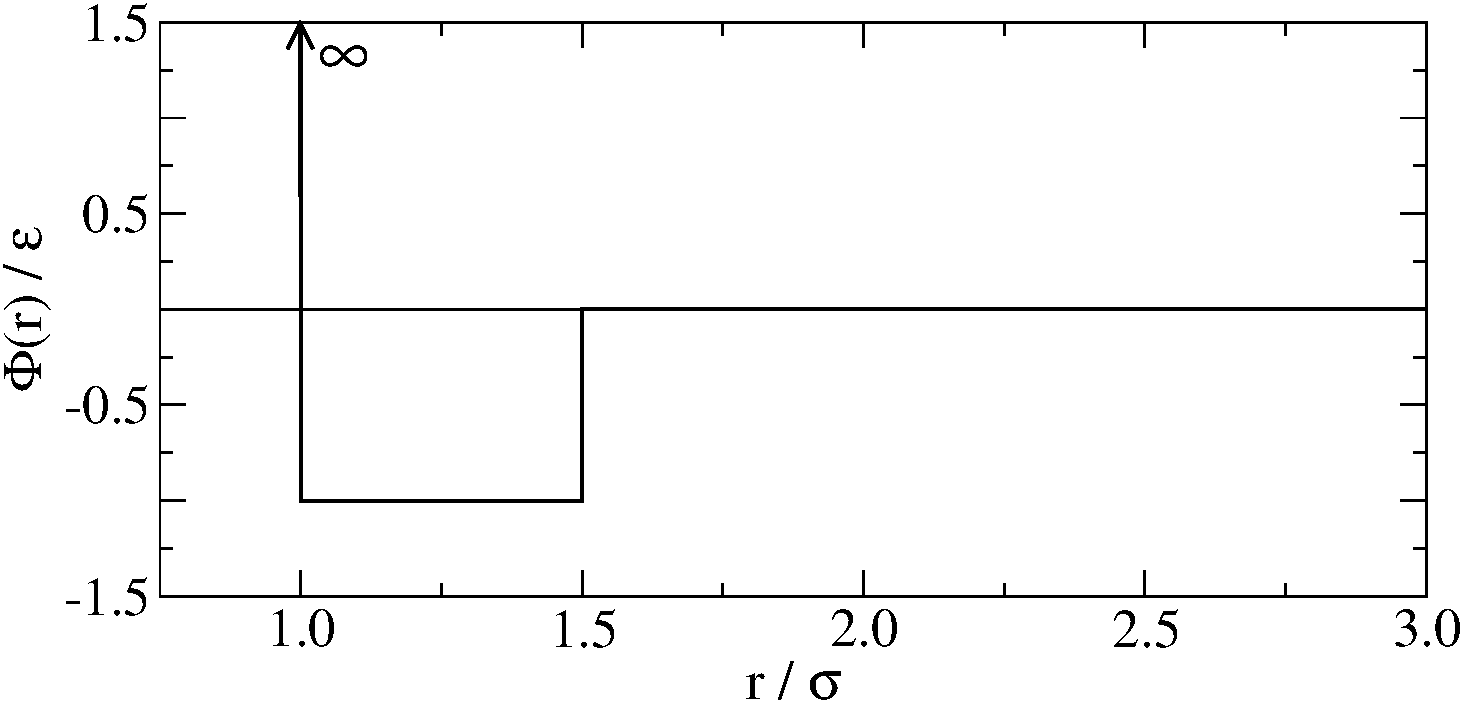
\includegraphics[clip,scale=0.45]{figures/squareWell} 
    \caption{\label{fig:squareWell} Plot of the square well potential
      with $\lambda = 1.5$}
  \end{center}
\end{figure}

Stepped potentials are a combination of square wells and square
shoulders to mimic the behaviour of a continuous potential.  Many
types of stepped potentials have been developed in the literature.
Chapela \textit{et al.} \cite{Chapela1989} created a stepped version
of the Lennard-Jones potential shown in Figure \ref{fig:chapelasteps}.

\begin{figure}[htp] 
  \begin{center}
    \includegraphics[clip,scale = 0.45]{figures/ChapelaSteps} 
    \caption{\label{fig:chapelasteps} A stepped version (solid line) of the
      continuous Lennard-Jones potential (dashed line) created by Chapela
      \textit{et al.}}
  \end{center}
\end{figure}

The SPEADMD (Step Potentials for Equilibria and Discontinuous
Molecular Dynamics)\nomenclature[A]{SPEADMD}{Step Potentials for
  Equilbria and Discontinuous Molecular Dynamics} project has created
stepped potentials that represent a range of hydrocarbons
\cite{ElliotJr2002, Unlu2004, Vahid2010}.  These potentials
have been converted to equations of state that match experimental
values relatively well.

\begin{figure}[htp] 
  \begin{center}
    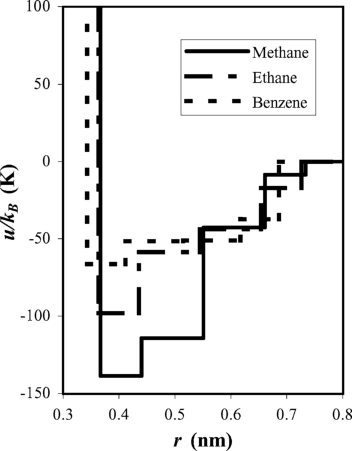
\includegraphics[clip,scale = 1.2]{figures/SPEADMD} 
    \caption{\label{fig:SPEADMD} SPEADMD stepped potentials for
      methane, ethane and benzene \cite{ElliotJr2002}.}
  \end{center}
\end{figure}

Stepped potentials have also been used to model protein interactions
using PRIME.

% Hard sphere,
%
%square well -> compare to LJ
%
%SPEAMD, PRIME
%
%Lead out with the two methods used to simulate these potentials are quite different....


\chapter{Molecular Dynamics}

\section{Applying Classical Mechanics to Molecules}
%OR SOMETHING SIMILAR
%% Start with F=MA again, talk about how to solve it.

The most fundamental part of molecular dynamics is solving Newton's
Second Law of Motion (Eq.~\eqref{eq:Fmrddot}).

\begin{equation} 
  \mathbf{F} = m \frac{\partial^2 \mathbf{r}}{\partial t^2}
  \label{eq:Fmrddot} 
\end{equation}

While the forces acting on the particles can be calculated from their
intermolecular potentials, the future positions of the particles
become the solution of a differential equation.  The techniques used
to solve this differential equation are different depending on
whether the potential is continuous or discontinuous.

\section{Force-Driven Simulation}
\subsection{Introduction}
For continuous potentials it is not possible to solve for the
particle's future position analytically.  This because the force is
not constant so the differential equation has an infinite number of
derivatives.  Therefore numerical methods for solving differential
equations have to be used; these are known as integrators.

\subsection{Integrators} 

The majority of numerical integrators are based on Taylor Series
(Eq.~\ref{eq:Taylor}).

\begin{equation} 
\mathbf{r}(t+\Delta t) = \mathbf{r}(t) + 
\frac{\partial\mathbf{r}(t)}{\partial t}(\Delta t) + 
\frac{1}{2}\frac{\partial^2\mathbf{r}(t)}{\partial t^2}\Delta t^2 + 
\frac{1}{3!}\frac{\partial^3\mathbf{r}(t)}{\partial t^3}\Delta t^3 
+ \frac{1}{4!}\frac{\partial^4\mathbf{r}(t)}{\partial t^4}\Delta t^4 
+ ... \label{eq:Taylor} 
\end{equation}

The simplest integrator is Euler's Method which is just the Taylor
Series truncated after the acceleration term (Eq.~\ref{eq:Euler}).

\begin{equation} 
  \mathbf{r}(t+\Delta t) = \mathbf{r}(t) + \mathbf{v}(\Delta t) +
  \frac{1}{2}\mathbf{a}\Delta t^2 
  \label{eq:Euler}
\end{equation}

However this method suffers from large errors and is highly unstable
(i.e.\ it amplifies any errors) \cite{Haile1997} and is therefore
rarely used. The Verlet Integrator \cite{Verlet1967} improves upon
Euler's method by combining the forward timestep with a reverse
timestep (Eq.~\eqref{eq:Verletpos}). This method is actually third
order as the third (and first) derivative is cancelled out during its
derivation. The Verlet integrator does not include an equation to
calculate the future velocity, as knowledge of the velocity is not
required for the integrator.  However it is often desired to know
velocities to calculate physical properties so the central difference
used by Verlet is often used to calculate velocities
(Eq.~\eqref{eq:VerletVel}).

\begin{subequations} 
  \begin{align} 
    \mathbf{r}(t + \Delta t) &= 2\mathbf{r}(t) - \mathbf{r}(t - \Delta t) 
    + \mathbf{a}(t)\Delta t^2
    \label{eq:Verletpos} \\
    \mathbf{v}(t+\Delta t) &= \frac{\mathbf{r}(t+\Delta t) -
      \mathbf{r}(t-\Delta t)}{2\Delta t} 
    \label{eq:VerletVel} 
  \end{align}
\end{subequations}

Integrators suffer from two key failings that cause a systematic gain
of energy known as ``energy drift''. Firstly, integrators are based on
infinite Taylor series which cannot be fully implemented and have
to be truncated after a certain number of terms; this introduces an
error. Secondly, integrators are unable to predict values of forces
that have discontinuities in them, such as discrete potentials or
discontinuities introduced by truncating potentials to improve
simulator speed.  There are a couple of types of integrators that try
and reduce these problems.

The first method to improve the traditional integrator is the
predictor-corrector integrator. These use a truncated Taylor series
to calculated a predicted value for the future position and higher
order time derivatives. The force is then calculated at this
predicited position, then the difference between the predicted
acceleration and the corrected acceleration calculated from the force
is used to correct the position and time derivatives.

The most popular predictor-corrector integrator is that of Gear
\cite{Gear1971} using the 5th order algorithm. The predicted value for
the $n^{th}$ time derivative is shown in
Eq.~\eqref{eq:GearPredictor}. By defining $\Delta \mathbf{a} =
\mathbf{a}\,^{C} - \mathbf{a}\,^{P}$, where the superscripts $C$ and
$P$ denote the corrected and predicted values respectively, the
corrected time derivatives can be calculated using
Eq.~\eqref{eq:GearCorrector} with coefficients from
Eq.~\eqref{eq:GearCoeff}.

\begin{equation} 
  \frac{\partial^{n}}{\partial t^{n}} \mathbf{r}\:^{P}(t+\Delta t)
  =\sum^{5}_{k=i} \frac{1}{k!}\frac{\partial^{n} }{\partial t^{n}}
  \mathbf{r}(t) \Delta t^{k} 
  \label{eq:GearPredictor} 
\end{equation}

\begin{equation} 
  \frac{\partial^{n}}{\partial t^{n}} \mathbf{r}\:^{C}(t+\Delta t)
  =\frac{\partial^{n} }{\partial t^{n}} \mathbf{r}\:^{P}(t+\Delta t)
  +\frac{c_i}{\Delta t^i} \left(\frac{\Delta t^2}{2}\Delta \mathbf{a}\right)
  \label{eq:GearCorrector} \end{equation} \begin{equation} c_0 =
  \frac{3}{16},\;\;c_1 = \frac{251}{360},\;\; c_2 = 1,\;\; c_3 =
  \frac{11}{18},\;\; c_4 =
  \frac{1}{6},\;\; c_5 = \frac{1}{60} \label{eq:GearCoeff} 
\end{equation}

Gear's algorithm, while more accurate at short timesteps than
Verlet's integrator \cite{Haile1997}, loses precision at long
timesteps and is computationally expensive.

The other method used to try and mitigate the failings of other types
of integrator is the sympletic integrator.  These have the useful
property in that they, on average, conserve energy
\cite{Hairer2003}. The most common symplectic integrator used in MD is
the Velocity Verlet Integrator \cite{Swope1982} shown in
\eqref{eq:VVerlet}.

\begin{subequations}
\label{eq:VVerlet}
\begin{align}
 \mathbf{r}(t + \Delta t) &= \mathbf{r}(t) + \mathbf{v}(t) \Delta t 
 + \frac{1}{2}\mathbf{a}(t) \Delta t^2
 \label{eq:VVerletpos} \\
 \mathbf{v}(t+\Delta t) &= \mathbf{v}(t) + \frac{\mathbf{a}(t) 
   + \mathbf{a}(t+\Delta t)}{2}\Delta t
 \label{eq:VVerletVel}
\end{align}
\end{subequations}

The popularity of the Velocity Verlet is due to its computational
simplicity and its accuracy and stability at relatively long
timesteps. It can even be expanded \cite{Khakimov2002} to maintain its
accuracy and stability at very long timesteps at a small extra
computational cost. However the Velocity Verlet cannot be used in
systems that do not conserve energy, i.e.\ systems with dissipative
forces.
\section{Event-driven Simulation}

\subsection{Introduction} 
The methods for integrating continuous potentials rely on calculating
the forces acting on the particles, however this is problematic when
working with discrete potentials.  The gradient (and hence the force) is
either infinite at the steps or zero between them.

Therefore a new technique for simulating these discrete potentials is
needed.  There is no force between the steps therefore the
acceleration (and higher order time derivatives) are zero and the
Taylor series (equation \eqref{eq:Taylor}) can be reduced to equation
\eqref{eq:edNewPos}.  

\begin{equation}
  \mathbf{r}(t+\Delta t) = \mathbf{r}(t) + \mathbf{v}(t)\Delta t 
  \label{eq:edNewPos}
\end{equation}

This allows the prediction of when particles reach a step, and using
the conservation of energy and momentum, the post collision velocities
of the particles can be calculated (this is expanded upon in section
\ref{sec:CollDyn}).  This method is known as event-driven molecular
dynamics and it is an analytical solution of Newton's Second Law of
Motion.

\subsection{Collision Time Prediction}
The prediction of the future positions of the particles using
Eq.~\eqref{eq:edNewPos} requires the time before the next
discontinuity is reached by any pair of particles. This section
outlines how these collision times are calculated.

For hard sphere simulations there are two conditions that must be
satisfied in order for a collision to occur.  Firstly, the particles
must be moving towards each other and secondly, the particles must
pass close enough to each other to collide.  These conditions can be
expressed mathematically in equations \eqref{eq:collConditions1} and
\eqref{eq:collConditions2} respectively \cite{Haile1997}.

\begin{subequations}
  \begin{align}
    \mathbf{v}_{ij}\cdot\mathbf{r}_{ij} < 0 \label{eq:collConditions1}\\
    (\mathbf{v}_{ij}\cdot\mathbf{r}_{ij})^2 
    - v_{ij}^2(r_{ij}^2 - \sigma^2) \geq 0 \label{eq:collConditions2}
  \end{align}
\end{subequations}

The time to collision can then be calculated using the quadratic in
equation \eqref{eq:collEnterTime}.  While there are two solutions,
only the earliest collision (the negative root) needs to be
considered.  The second root gives the time when the particles leave
after passing through each other which, for hard sphere, cannot
happen.

\begin{equation}
\Delta t = \frac{(-\mathbf{v}_{ij}\cdot\mathbf{r}_{ij}) \pm 
  \sqrt{(\mathbf{v}_{ij}\cdot\mathbf{r}_{ij})^2 - v_{ij}^2(r_{ij}^2 - \sigma^2)}}
       {v_{ij}^2} \label{eq:collEnterTime}
\end{equation}

Since $\mathbf{v}_{ij}\cdot\mathbf{r}_{ij}$ must be negative for the
collision, there is the possibility of catastrophic cancellation
\cite{Goldberg1991}, if $(\mathbf{v}_{ij}\cdot\mathbf{r}_{ij})^2 \gg
v_{ij}^2(r_{ij}^2 - \sigma^2)$. Therefore it is advisable to use the
positive root from the alternate form of the quadratic equation given
in equation \eqref{eq:collEnterTimeAlt} \cite{Poschel2005}.

\begin{equation}
\Delta t = \frac{r_{ij}^2 - \sigma^2}{(-\mathbf{v}_{ij}\cdot\mathbf{r}_{ij})
  \mp \sqrt{(\mathbf{v}_{ij}\cdot\mathbf{r}_{ij})^2 
    - v_{ij}^2(r_{ij}^2 - \sigma^2)}}
\label{eq:collEnterTimeAlt}
\end{equation}

When considering stepped potentials many of the same principles apply,
except there are now two possible ``collisions''. The first, when two
particles enter a step is treated identically to hard spheres. The
other event, when the particles leave the step, is calculated using
the second, later root of the quadratic.  In order to prevent loss of
numerical precision, the leaving time should be calculated using
equation \eqref{eq:collExitTime}.

\begin{equation}
  \label{eq:collExitTime}
\Delta t = 
\begin{cases}
  \frac{r_{ij}^2 - \sigma^2}{(-\mathbf{v}_{ij}\cdot\mathbf{r}_{ij})
    - \sqrt{(\mathbf{v}_{ij}\cdot\mathbf{r}_{ij})^2 
      - v_{ij}^2(r_{ij}^2 - \sigma^2)}}, & \text{if }
  \mathbf{v}_{ij}\cdot\mathbf{r}_{ij} > 0 \\
\\

\frac{(-\mathbf{v}_{ij}\cdot\mathbf{r}_{ij}) +
  \sqrt{(\mathbf{v}_{ij}\cdot\mathbf{r}_{ij})^2 - v_{ij}^2(r_{ij}^2 - \sigma^2)}}
     {v_{ij}^2} , & \text{if }
     \mathbf{v}_{ij}\cdot\mathbf{r}_{ij} < 0 
\end{cases}
\end{equation}

\subsection{Collision Dynamics \label{sec:CollDyn}}
Once the time of the next collision is known, the particles can be
moved to their new locations, using Eq.~\eqref{eq:edNewPos}. However,
in order to predict future collisions the post-collision velocities of
the colliding particles must also be calculated.  

The simplest collision between two particles is an elastic bounce,
where the velocities and just exchanged along the separation vector
between the two particles.  The change in velocity during the
collision for particles $i$ and $j$ is shown in
Eq.~\eqref{eq:postVBounce}.

\begin{subequations}
  \label{eq:postVBounce}
  \begin{align}
    \Delta\mathbf{v}_i &= -(\mathbf{v}_{ij}\cdot\mathbf{\hat{r}}_{ij})\mathbf{\hat{r}}_{ij} \\
    \Delta\mathbf{v}_j &= (\mathbf{v}_{ij}\cdot\mathbf{\hat{r}}_{ij})\mathbf{\hat{r}}_{ij}
  \end{align}
\end{subequations}

For stepped potential system, the collision dynamics are more complex.
When two particles collide they must pay an energy ``cost'' to proceed
through the step.  This energy cost $\Delta \Phi$ is the difference in
the energy of the current step and the step the particles are going
into, and is shown in Eq.~\eqref{eq:energyCost}.

\begin{equation}
  \label{eq:energyCost}
  \Delta \Phi = U_{\text{next step}} - U_{\text{current step}}
\end{equation}

If the kinect energy of the particles is insufficient, the pair bounce
off the step and the post-collision velocities are calculated using
equation \eqref{eq:postVBounce}. However, if the particles can pay
this cost i.e.\ the inequality \eqref{eq:kineticCost} is true, then the
particles can enter the step.

\begin{equation}
\label{eq:kineticCost}
  \frac{1}{4}m(\mathbf{v}_{ij}\cdot\mathbf{\hat{r}}_{ij})^2 > \Delta \Phi
\end{equation}

The change in the velocities of particles $i$ and $j$ after going
through a step are shown in equation \eqref{eq:postVCapture} where $A$
is given in equation \eqref{eq:changeMomentum}, the derivation of
these equations is given in Appendix \ref{app:derivation}.  If the
particles are entering a step, the positive root of $A$ is used,
whereas if the particles are leaving a step it is the negative root
that should be used.

\begin{subequations}
  \label{eq:postVCapture}
  \begin{align}
    \Delta\mathbf{v}_i &= \frac{A}{m} \mathbf{\hat{r}}_{ij} \\
    \Delta\mathbf{v}_j &= -\frac{A}{m}\mathbf{\hat{r}}_{ij}
  \end{align}
\end{subequations}

\begin{equation}
  \label{eq:changeMomentum}
  A = -\frac{m}{2}\left((\mathbf{v}_{ij}\cdot\mathbf{\hat{r}}_{ij}) \pm
  \sqrt{(\mathbf{v}_{ij}\cdot\mathbf{\hat{r}}_{ij})^2 - \frac{4}{m}\Delta \Phi}\right)
\end{equation}

It can be noticed that Eq.~\eqref{eq:postVBounce} can be derived from
Eqs.~\eqref{eq:postVCapture} and \eqref{eq:changeMomentum} by setting
$\Delta \Phi=0$.

 \newpage
\section{Force-driven Simulators} 
In order to compare the effectiveness of step potentials a set of
comparison results from a continuous potential is needed.  The method
to simulate a continuous potential is given in this section.

Force-driven (or time driven) simulators are the most popular method
of simulating particles due to their relative simplicity and ability
to handle continuous potentials. Simulators of this kind were
pioneered by Rahman \cite{Rahman1964} who predicted physical
properties of liquid argon using a Lennard-Jones potential with
reasonable accuracy.

The distinguishing feature between force-driven and event-driven
simulators is the way in which they move through time. During
force-based simulations particles' positions and velocities are
calculated at uniform intervals of time, $\Delta t$ using the forces
acting on the particles. These newly calculated values are then used
to predict the next set of particle positions. This is then repeated
over the desired simulation time.

The general algorithm for a force driven simulator is as follows:
\begin{flushleft}
  \begin{enumerate} 
  \item Initialisation 
  \item Calculate particles' future positions 
  \item Calculate the forces acting on the particles 
  \item Calculate the future velocities of particles 
  \item Run thermostat (if enabled) 
  \item Measure properties 
  \item Repeat steps 2-6 for the desired number of iterations
  \end{enumerate} 
\end{flushleft}

\subsection{Initialisation \label{sec:initMD}} 
The particles are initialised in a Face Centered Cubic (FCC)
\nomenclature[A]{FCC}{Face Centered Cubic} structure. The use of the
FCC lattice is common when simulating Lennard-Jones potentials as the
first force-driven simulation \cite{Rahman1964} was carried out using
liquid Argon which crystalises to a FCC lattice.

Particle velocities are assigned randomly from a Gaussian distribution
with a mean, $\mu = 0$, and a standard deviation, $\sigma =
\sqrt{T^{*}}$, where $T^{*}$ is the desired reduced temperature. The
velocities are then rescaled to ensure there is no net shift in linear
momentum in any direction by applying \eqref{eq:zeroLinearP} in each
orthongonal direction.

\begin{equation} 
  v_{i}^{new} = v_{i}^{old} - \frac{1}{N}
  \sum^{N}_{i}v_{i}^{old}
  \label{eq:zeroLinearP} 
\end{equation}



In this disseration the Velocity Verlet integrator is used as all
forces are conservative.

\subsection{Periodic Boundary Conditions}

When simulating a system it is necessary to have a boundary to prevent
the particles from moving away from each other into infinity.  However
solid walls have a large effect on the properties of a system so an
alternative method is needed.  Since the earliest MD simulations
\cite{Alder1959} have used periodic boundary conditions to solve this
problem.

The concept behind periodic boundary conditions is to create a
pseudoinfinite system made up of tessellated images of the simulated
system (as shown in figure \ref{fig:PBC}).  When a particle leaves the
primary cell, its image enters from the opposite side.  This ensures
mass is conserved in each cell.  This, however, brings the problem of
particles being able to interact with multiple images of another
particle, or even with themselves.  The minimum image criterion is
used to ensure particles only interact with the closest image of
another particle.

\begin{figure}[htp] 
  \begin{center}
    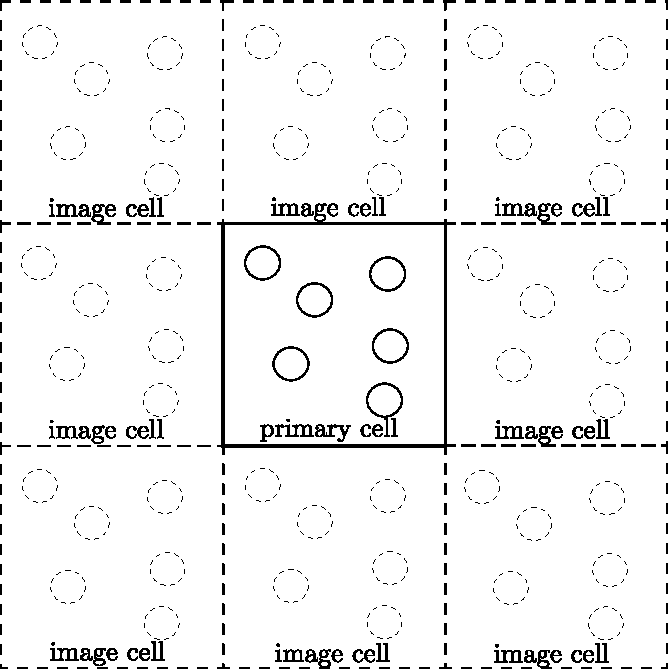
\includegraphics[clip, scale = 0.8]{figures/PBC} 
    \caption{\label{fig:PBC} Figure showing 2D periodic boundary
      conditions. Only the nearest 8 images (dashed) to the simulated
      system (solid) are shown.}
  \end{center}
\end{figure}

\subsection{Thermostat}

All simulations in this dissertation used the caniocal NVT ensemble,
i.e.\ the number of particles, $N$; the volume of the system, $V$ and
the temperature, $T$ were kept constant during the simulation.  While
keeping the number of particles and system size constant is simple,
controlling the temperature is more complex.  

The simplest method for controlling the temperature is to rescale the
particle velocities to match the desired temperature using equation
\eqref{eq:tempRescale}. 

\begin{equation}
  \label{eq:tempRescale}
  \mathbf{v}_{\text{new}} = \mathbf{v}_{\text{old}} \sqrt{\frac{T_{\text{desired}}}{T_{\text{current}}}}
\end{equation}

However this does not allow energy fluctuations that should exist in a
NVT system, therefore an Andersen thermostat\cite{Andersen1980} is
used.  An Andersen thermostat works by colliding a random particle
with a ghost particle at the desired temperature.  In this
force-driven simulation, this is achieved by reassigning the
velocities of 5\% of particles from a Gaussian distribution at the
correct temperature (similar to section \ref{sec:initMD}).

\subsection{Optimisation \label{sec:Optimisation}}

Due to the time-consuming nature of computer simulations there are a
number of techniques used to speed up simulations.  Since the
calculation of the forces on the particles is the most time-consuming
part of force-driven simulations \cite{Frenkel2002}, almost all
optimising techniques focus on this aspect.

The first technique to improve simulation speed is to truncate the
potential.  Since continuous potentials tend to zero as particles get
further away from each other, significant time can be saved by
selecting a cut-off radius at which the potential is taken to be zero.
The form of a truncated potential is shown in equation
\eqref{eq:truncatePotential}.  For the Lennard-Jones potential a
cut-off radius of $3\sigma$ is used as $\Phi(3\sigma) =
-0.00548\varepsilon$ and $F(3\sigma) = -0.0109\varepsilon/\sigma$ are
both approximately 0.5\% of the minimum values.

\begin{equation}
  \label{eq:truncatePotential}
  \Phi(r) = 
  \begin{cases}
    \Phi(r) &\text{if }\; r \leq r_{\text{cut-off}} \\
    0 & \text{if }\; r > r_{\text{cut-off}} 
  \end{cases}
\end{equation}

While truncating the potential prevents the calculation of the forces
it still requires the computation of the distance between particles.
These extraneous calculations can be eliminated by using a neighbour list.

There are two main types of neighbour list used in molcular dynamics
simulations.  The first is the use of Verlet lists \cite{Verlet1967},
and this is the type used in this disseration for the force-driven
simulation.  A Verlet list is a list of all the particles within a
certain radius of a particle.  If this list was updated every
timestep, this would be no improvement on the original method, but by
making the Verlet radius larger than the truncation radius, these list
can be used for multiple timesteps.  Haile \cite{Haile1997} recommends
using a Verlet radius of $3.3\sigma$, and updating the list every $10$
timesteps, and this is what was done in this dissertation.

Another method is to use cell-linked lists \cite{Poschel2005}, this
method involves dividing the system into a grid and only the particles
in the same cell or a neighbouring cell are taken into account.  This
method can however be inefficient as the length of each cell must be
at least the truncation cut-off radius wide to prevent particles being
missed out.  However this means a volume of $27r_{\text{cut-off}}^3$
(as in 3 dimensions each cell has 26 neighbours) are considered but
only particles within the spherical volume $\frac{4}{3}\pi
r_{\text{cut-off}}^3$ should be checked; this means the volume checked
is over six times larger than it needs to be.  

Mattson and Rice \cite{Mattson1999} improve this by reducing the
length of each cell to less than the cut-off radius, but this results
in more neighbouring cells having to be checked i.e. for a cell length
of $0.5r_{\text{cut-off}}$ the nearest 124 (a $5\times 5\times 5$
grid) cells are considered neighbours. This means there is a
compromise as smaller cells mean that less volume is checked, but also
means the cell lists are made obsolete quicker and therefore have to
generated more frequently.

\section{Event-Driven Simulators}

Though force-driven simulators are more popular the first MD
simulation was done using an event-driven simulator by Alder and
Wainwright \cite{Alder1957}. Event-driven simulators differ from
force-driven simulators in that they move through time by jumping from
the point when a discontinuity occurs (known as a collision) to the
next discontinuity.  These collisions are taken to be instantaneous
and only one can occur at any particular time.

The general algorithm for a event driven simulator shown below.

\begin{flushleft}
  \begin{enumerate} 
  \item Initialisation 
  \item Find the next event
  \item Process the event
  \item Update the event list
  \item Measure properties 
  \item Repeat steps 2-5 for the desired number of events
  \end{enumerate} 
\end{flushleft}

\newpage

\chapter{Measuring Thermodynamic Properties}
\section{Introduction}
Molecular dynamics is a useful tool to predict macroscopic properties
of particles systems.  Many of the identities and methods to measure
these properties are derived in statistical mechanics.  However, even
when the system is at equilibrium, these properties fluctuate around a
mean (see Figure \ref{fig:fluctuations}) therefore it is common to
take time averages of these values. These time averages are denoted
with angle brackets $\langle\:\: \rangle$, and the time average of a
property, $A$, is shown in \eqref{eq:TAdef} \cite{Haile1997}.

\begin{figure}[htp] 
  \begin{center}
    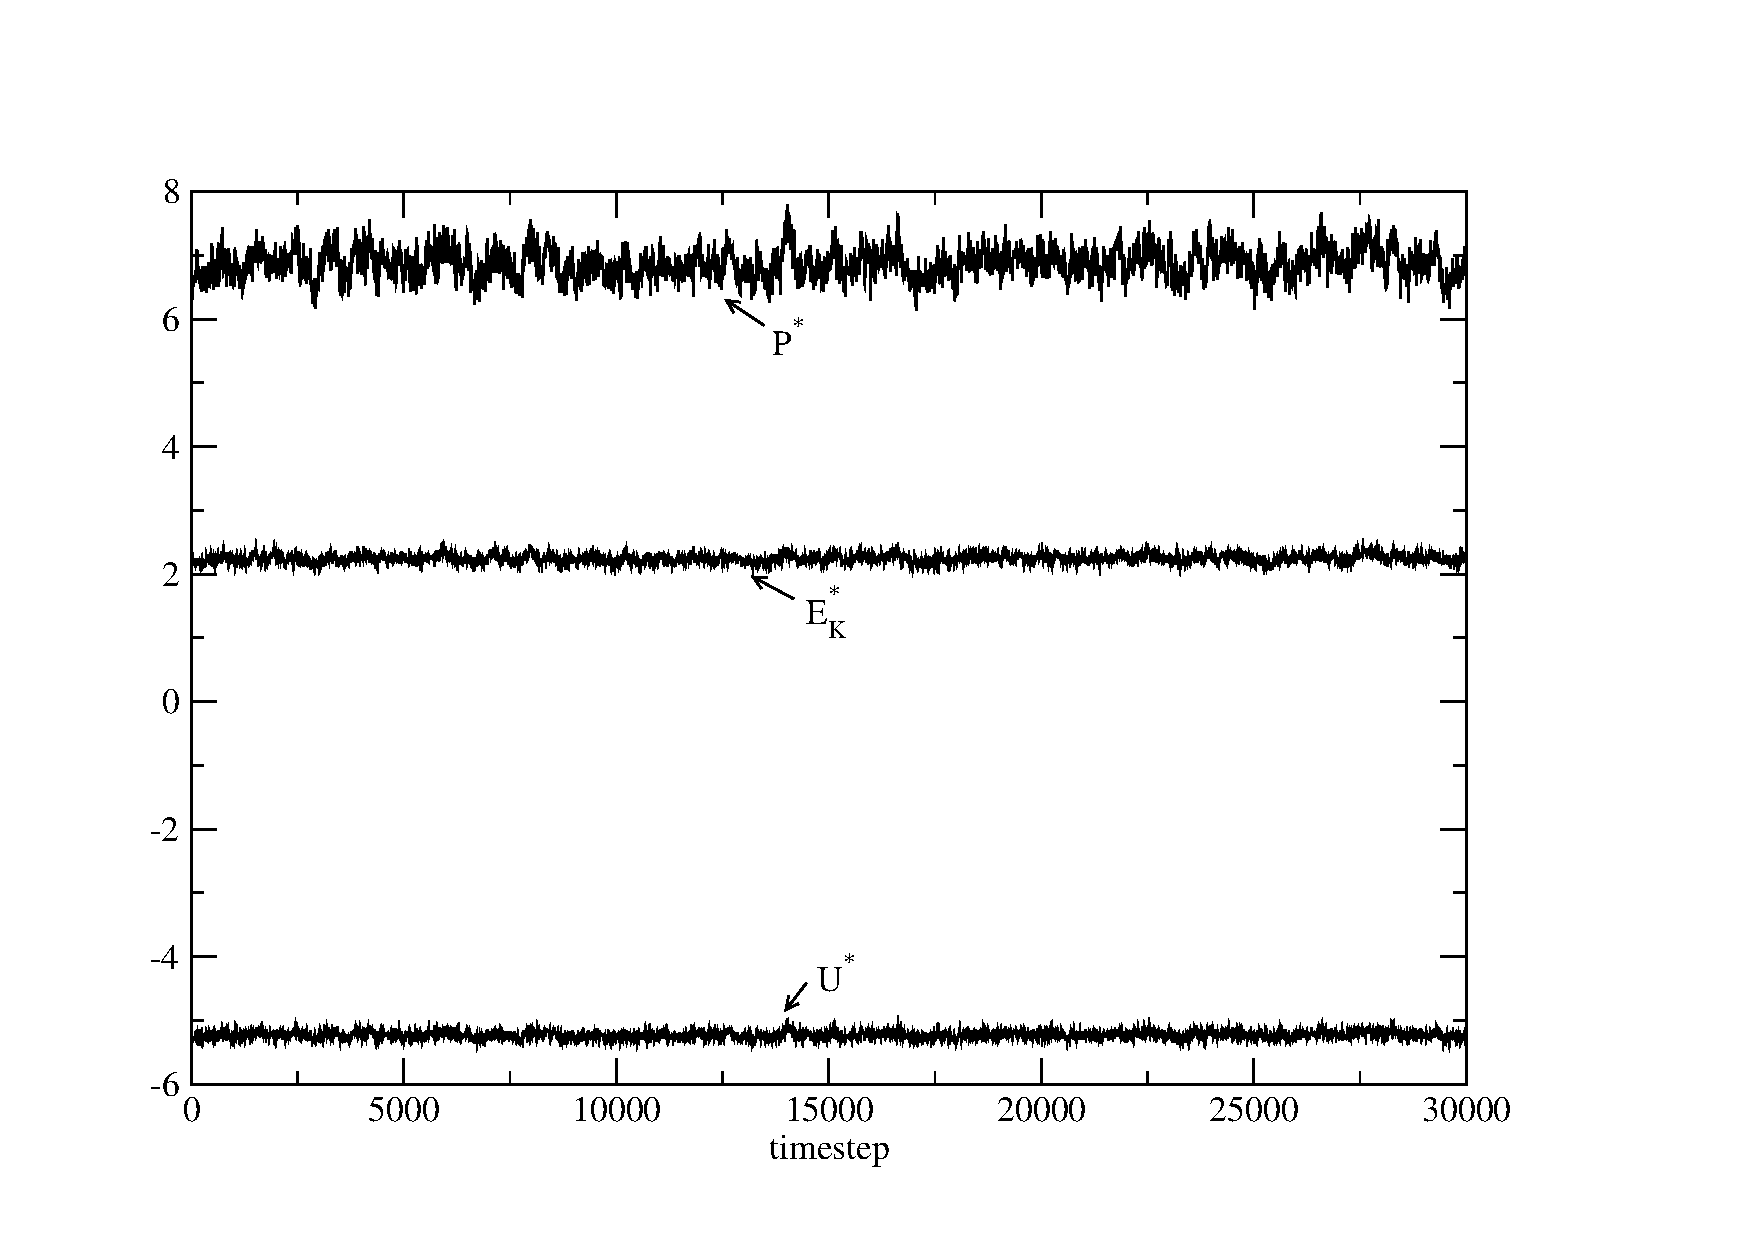
\includegraphics[clip,width=\textwidth]{figures/energyplot} 
    \caption{\label{fig:fluctuations} Plot showing flucuation of pressure
      ($P^*=P\sigma^3/\varepsilon$), kinetic energy per particle
      ($E_K^*=E_K/N\varepsilon$) and potential energy per particle
      ($\Phi^*=U/N\varepsilon$).  Results are from a force-driven simulation
      involving 864 particles, at a density $\rho^*=0.9$ and
      temperature $\langle T^*\rangle=1.497$. Values were collected
      every 10 timesteps where each timestep was $\Delta t^* = 0.005$.}
  \end{center}
\end{figure}

\begin{equation}
  \label{eq:TAdef}
  \langle A \rangle = \lim_{t \to \infty} \frac{1}{t}  \int^{t_0+t}_{t_0}A(\tau) d\tau
\end{equation}

This time average can be calculated precisely in event-driven
simulations for several properties such as pressure, kinetic energy
and potential energy.  These only change at collisions and therefore
are constant for the time between the collision and can be calculated
by \eqref{eq:TASum}.

\begin{equation}
  \label{eq:TASum}
  \langle A \rangle = \frac{1}{t}\sum^{t_o+t}_{t_0}A(\tau)\Delta \tau
\end{equation}

In force-driven simulators all properties change continuously and
hence time averages cannot be calculated precisely, however
approximations can be made. If properties are measured every uniform
period of time, the time average can be approximated by equation
\eqref{eq:TAforcedriven}, where $M$ is the number of measurements
taken.

\begin{equation}
  \label{eq:TAforcedriven}
  \langle A \rangle = \frac{1}{M} \sum^{M}_{1}A(\tau)
\end{equation}
\section{Units}

In molecular dynamics simulations, properties are frequently measured
in dimensionless forms \cite{Haile1997}. These ``reduced units'' are
usually denoted with an asterisk.  In order to achieve this a number
of fundamental dimensions are needed: a characteristic length
$\sigma$, a characteristic energy $\varepsilon$, and the mass of one
particle $m$.  In the case of the Lennard-Jones potential, the
characteristic length and energy are taken as: the distance of the
root, and the depth of the attractive well respectively. A table of
reduced forms are given in table \ref{tab:reducedForms}.

\begin{table}[htp] 
  \caption{Table of reduced forms of various quanities used in this
    dissertation \cite{Haile1997}}
  \label{tab:reducedForms}
  \begin{center}
    \begin{tabular}{c c}
      \toprule
      Quantity & Reduced forms \\
      \midrule
      Density & $\rho^* = N \sigma^3 / V$ \\
      Energy & $U^* = U / \varepsilon$ \\
      Force & $F^* = F\sigma/\varepsilon$ \\
      Length & $r^* = r / \sigma$ \\
      Pressure & $P^* = P \sigma^3 /\varepsilon$ \\
      Temperature & $T^* = kT/\varepsilon$ \\
      Time & $t^* = t / (\sigma \sqrt{m/\varepsilon})$ \\
      Velocity & $v^* = v\sqrt{m/\varepsilon}$ \\
      \bottomrule
    \end{tabular}
  \end{center}
\end{table}

\section{Energy \label{sec:Energy}}
Perhaps one of the most important properties to measure in MD
simulations is the total internal energy of the system.  For isolated
systems, i.e.\ systems where mass or energy cannot enter or leave the
system, this internal energy is the sum of kinetic and potential
energy (equation \eqref{eq:internalE}).

\begin{equation}
  U = E_K + \Phi \label{eq:internalE}
\end{equation}

The total kinetic energy in the system is the sum of the kinetic
energy of each particle, as shown in equation \eqref{eq:totalEK}.

\begin{equation}
  \label{eq:totalEK}
  E_K = \sum_i^N mv_i^2
\end{equation}

The potential energy of the system is the sum of the potential energy
between every pair of particles (for a pairwise potential), and is
shown in equation \eqref{eq:totalU}.

\begin{equation}
  \label{eq:totalU}
  \Phi = \underset{i\;\;<\;\;j}{\sum\sum}\Phi(r_{ij})
\end{equation}

Event-driven simulators strictly conserve energy, therefore the
kinetic and potential energy can be measured at the beginning of the
simulation and then updated whenever either changes e.g.\ when a
collision occurs.

\section{Temperature}

The velocity distrubution of particles is given by the Maxwell
distribution \cite{Haile1997}, shown in equation
\eqref{eq:MaxwellDist}, where $k_B$ is the Boltzman Constant.

\begin{equation}
  \label{eq:MaxwellDist}
  f(v_x)dv_x = \sqrt{\frac{m}{2\pi k_BT}}e^{-\frac{mv_x^2}{2k_BT}} 
\end{equation}

This is the form of a Gaussian distribution and it can be shown
\cite{Landau1968} that the mean square velocity in any direction is as
shown in equation \eqref{eq:MSV}.

\begin{equation}
  \label{eq:MSV}
  \bar{\;v_x^2\;} = \frac{k_BT}{m}
\end{equation}

Making the assumption that the velocity distribution is the same in
each direction, the temperature can be expressed as equation
\eqref{eq:Temperature}, by taking the average temperature in each
direction. 

\begin{equation}
\label{eq:Temperature}
  T^* = k_BT = \frac{mv^2}{3N} = \frac{2}{3N}E_K
\end{equation}

This allows the calculation of the temperature from the kinetic energy
of the system.
\section{Pressure \label{sec:Pressure}}

The pressure in a molecular dynamics simulation is calculated using
the virial equation of state (equation \eqref{eq:virialEOS})
\cite{Landau1968}.

\begin{equation}
  \label{eq:virialEOS}
  \frac{PV}{Nk_BT} = 1 + B_2\rho + B_3\rho^2 + B_4\rho^3 + ...
\end{equation}

The coefficients, $B_2, B_3, B_4, ...$ are known as the second, third,
fourth, etc. virial coeffcients.  Values for these virial coefficients
are available in the literature for common potentials such as hard
spheres \cite{Labik2005} or Lennard-Jones
\cite{Schultz2009}. Physically these coefficients represent the
contribution to the pressure by two, three, four, etc. particles
interacting, and since most potentials are pairwise the pressure
contribution is truncated at the second virial coefficient, the form
of which in three dimensions is given in equation
\eqref{eq:secondVirial} \cite{Smith2005}.

\begin{equation}
  \label{eq:secondVirial}
  B_2 = -2\pi \int^\infty_0 \left(e^{\mathcal{U}(r)/kT}-1\right)r^2dr
\end{equation}

However these virial coefficients do not apply to molecular dynamics
simulations that use periodic boundary conditions \cite{Haile1997},
therefore an alternative method is required.

Using kinetic theory and measuring momentum flux during the simulation
an expression for the second virial coefficient can be created for
both simulation methods.  In force driven simulations, the second
virial can be calculated using equation \eqref{eq:virialMD}
\cite{Haile1997}.

\begin{equation}
  \label{eq:virialMD}
  B_2\rho = \frac{1}{3NkT}\left \langle\underset{i\;\;<\;\;j}{\sum\sum}\mathbf{F}_{ij}\cdot\mathbf{r}_{ij} \right\rangle
\end{equation}

Calculating the pressure in event-driven simulators is more complex
due to the lack of forces in the simulation, however by keeping track
of the momentum flux at each collision an average pressure can be
calculated using equation \eqref{eq:virialED}\cite{Lue2005}.  Here $N_{\text{coll}}$
is the total number of collisions during the time $t$.

\begin{equation}
  \label{eq:virialED}
  B_2\rho = \frac{m}{3}\frac{N_{\text{coll}}}{Nt}\langle\mathbf{r}_{ij}\cdot\Delta \mathbf{v}_i\rangle_{\text{coll}}
\end{equation}
\section{Radial Distrution Function}

One of the most important measurements in molecular dynamics is the
radial distribution function (RDF) \nomenclature[A]{RDF}{Radial
  Distribution Function}. The RDF provides information concerning the
arrangement of the particles, and can be determined experimentally
\cite{Yarnell1973}. This means that the RDF can be used to determine
the agreement of MD simulations and experimental results.

Statistically, the RDF is the ratio of the probability of finding a
particle a distance $r$ from another particle to the expected
probability if the particles were randomly distributed
~\cite{Allen1987}. Since potentials usually have a hard core there is
very little chance of finding a particle within the radius of another
particle, therefore the RDF is zero very close to the particle.
However as the radial distance tends to infinity the probability of
finding a particle tends to the randomly distributed probability so
the RDF tends to one, which can be seen in Fig.~\ref{fig:rdfsmooth}.

\begin{figure}[htp] 
  \begin{center}
    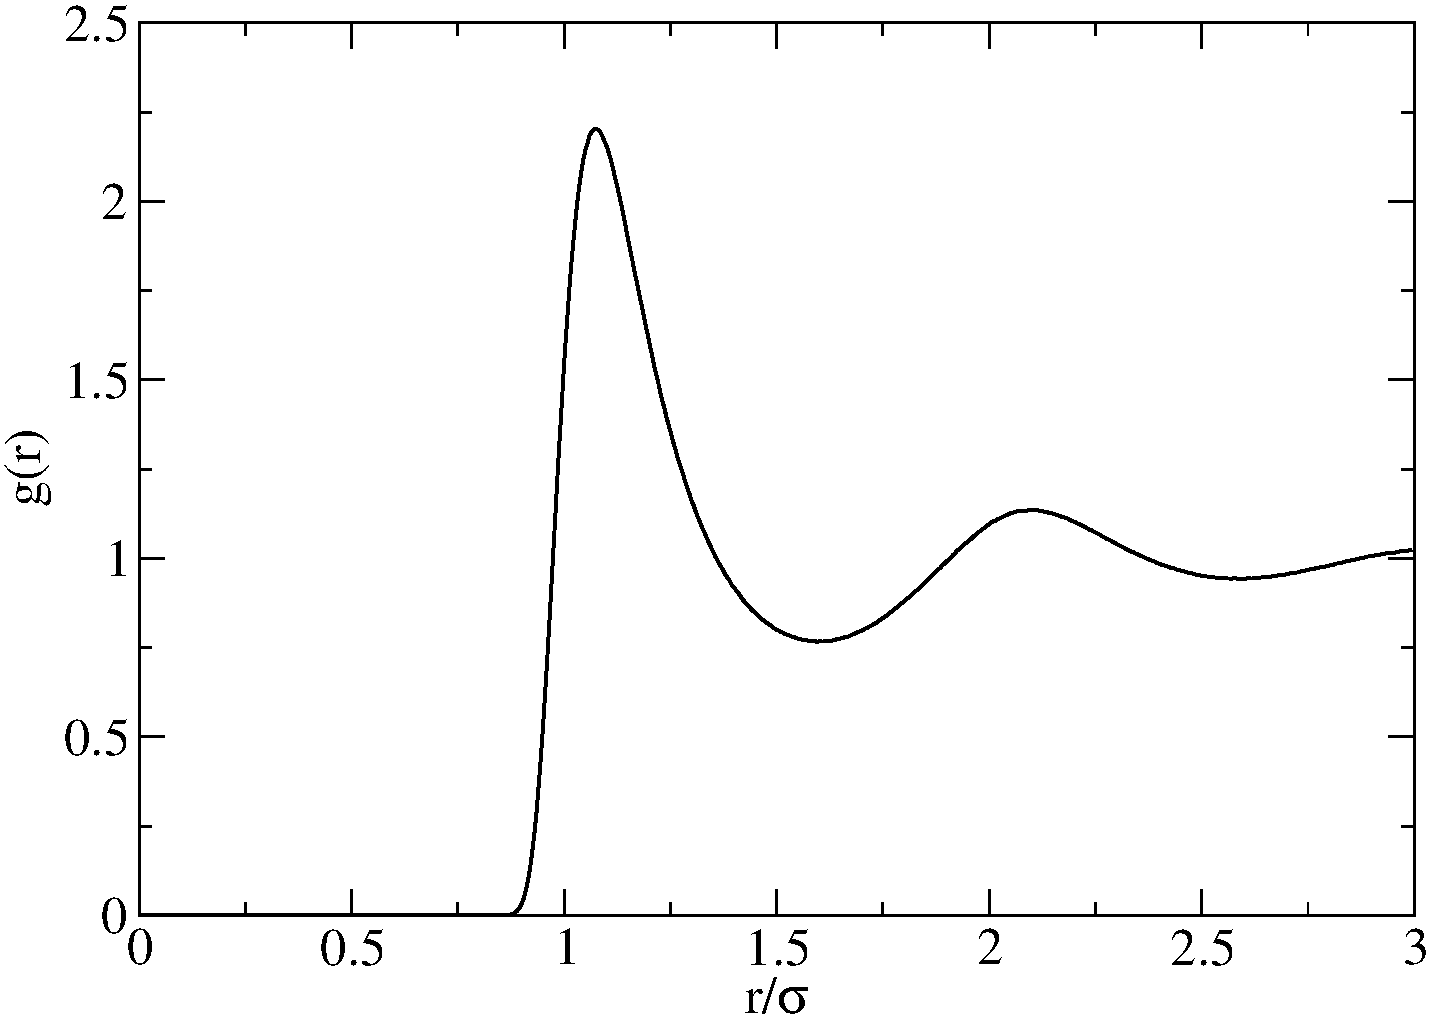
\includegraphics[clip,width=\textwidth]{figures/rdfsmooth} 
    \caption{\label{fig:rdfsmooth} Plot of the radial distribution
      function, $g(r)$, for a continuous Lennard-Jones
      potential. Results taken from a force-driven simulation at
      $\rho^*=0.7$ and $T^*=1.5$}
  \end{center}
\end{figure}

The RDF is measured in MD simulations by splitting the radial distance
into a number of bins.  The number of pairs of particles in a
particular bin is then counted.  The value of the RDF for bin $n$ can
be calculated using the following equation:

\begin{equation}
  \label{eq:rdf}
  g(n) = \frac{N_n}{NV_{\text{bin}}\rho}
\end{equation}

where $V_{\text{bin}}$ is the volume of the bin, and $N_n$ is the
number of particle pairs in bin $n$.  This measurement illustrates
another definition of the RDF.  The radial distribution function is
the ratio between the density at a specific distance from another
particle to the average density of the system.

Since the RDF contains information about the potential, simulations
with discrete potentials produce radial distribution functions with
discontinuities in them. Figure~\ref{fig:rdfrough} shows the RDF
produced when using the stepped potential shown in
Fig.~\ref{fig:chapelasteps}.

\begin{figure}[htp] 
  \begin{center}
    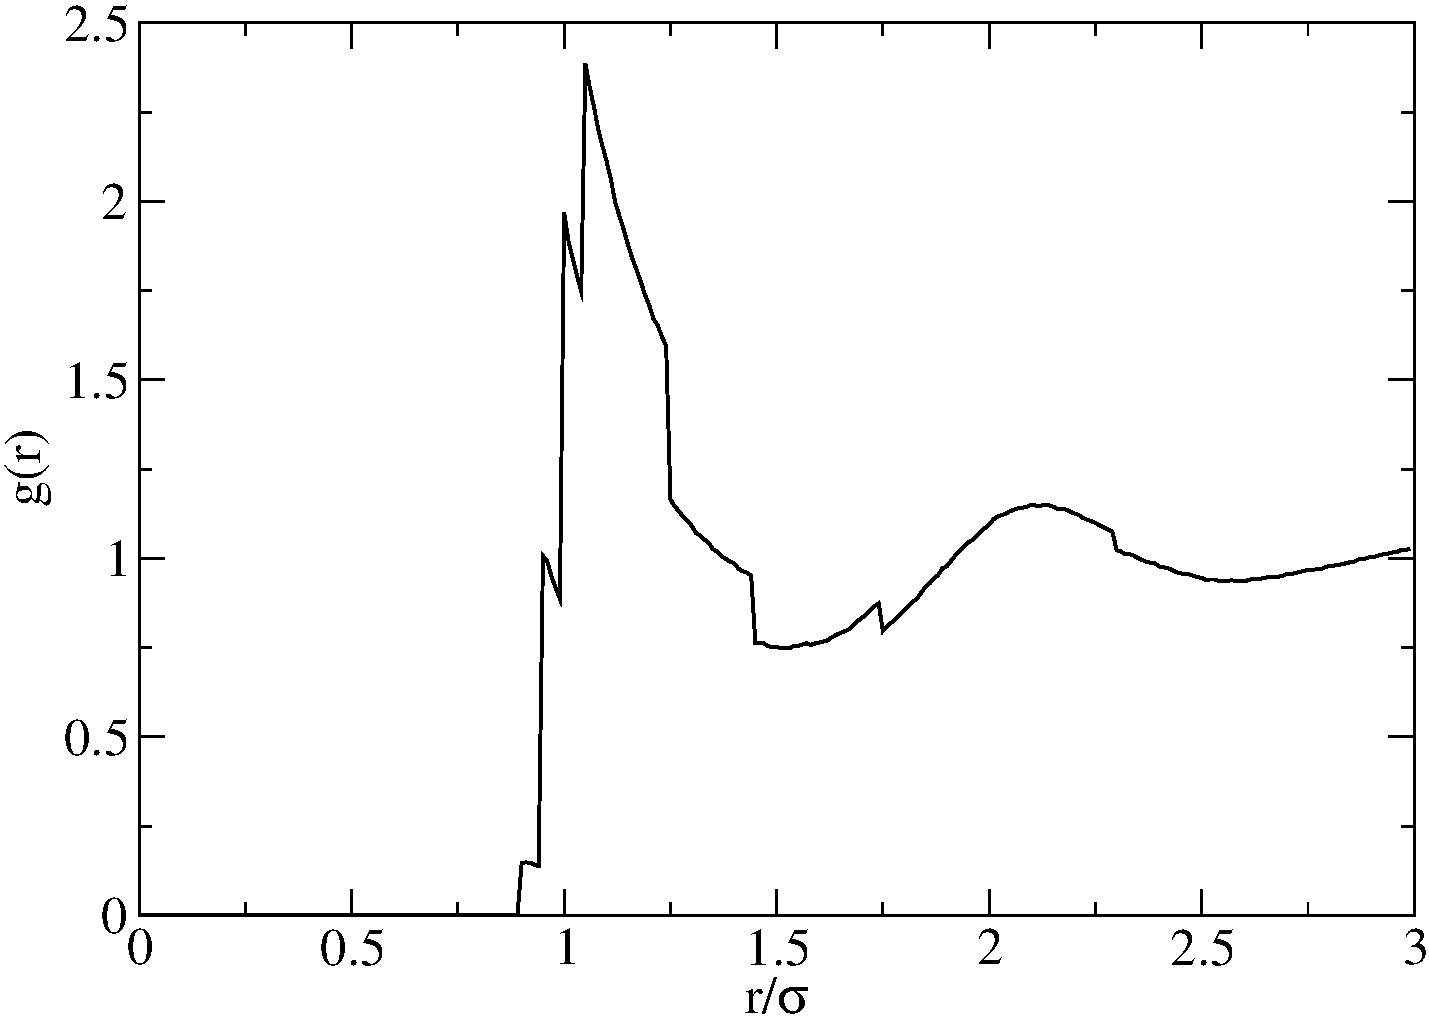
\includegraphics[clip,width=\textwidth]{figures/rdfrough} 
    \caption{\label{fig:rdfrough} Plot of the radial distribution
      function, $g(r)$, for a discrete stepped potential. Results
      taken from a event-driven simulation at $\rho^*=0.7$ and $T^*=1.5$}
  \end{center}
\end{figure}

This discontinuous RDF can be converted to a continuous function by
using the indirect correlation function, $y(r)$, \cite{Chapela1989}.
The indirect correlation function can be defined for both continuous
and discontinuous RDF and potentials using:

\begin{equation}
\label{eq:ICF}
y(r) = g_d(r)e^{\beta\Phi_d(r)} = g_c(r)e^{\beta\Phi_c(r)}
\end{equation}

where $\beta = 1/k_BT$ and the subscripts $c$ and $d$ denote the
continuous and discontinous functions respectively.  The continous
form of the RDF can then be calculated using
Eq.~\eqref{eq:continuousRDF}.  Figure~\ref{fig:rdfcomp} shows the
continuous form of the discontinuous RDF shown in
Fig.~\ref{fig:rdfrough}.

\begin{equation}
\label{eq:continuousRDF}
g_c(r)=g_d(r)e^{[\Phi_d(r)-\Phi_c(r)]\beta}
\end{equation}

\begin{figure}[htp] 
  \begin{center}
    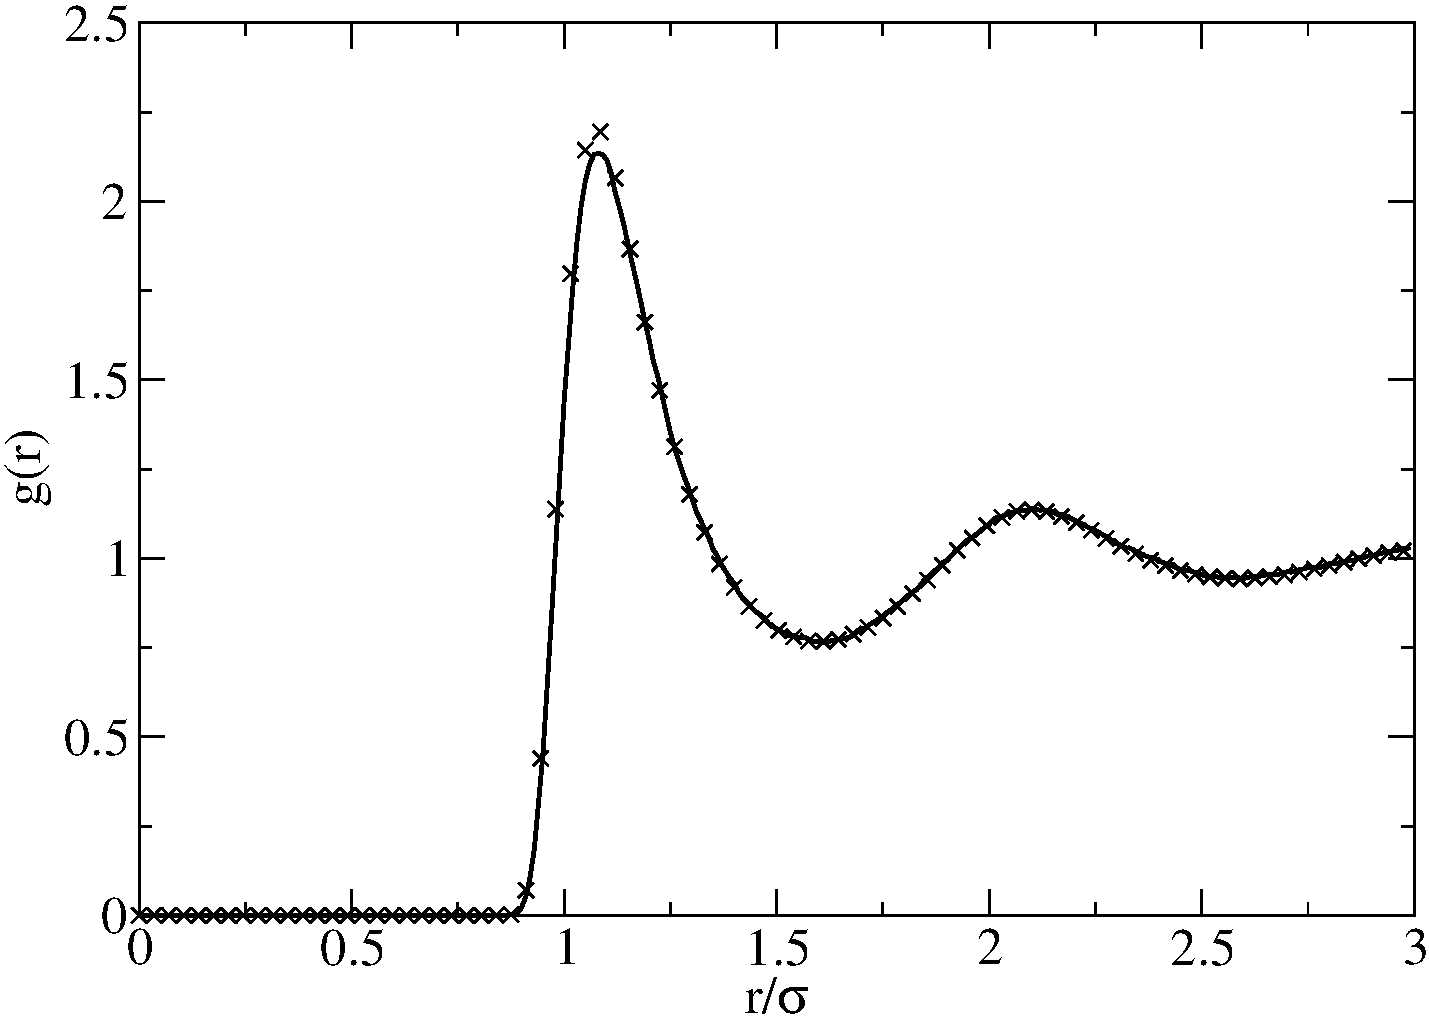
\includegraphics[clip,width=\textwidth]{figures/rdfcomp} 
    \caption{\label{fig:rdfcomp} The continuous form of the radial
      distribution function of a discrete potential is shown with the
      solid line.  The crosses show the RDF obtained from the
      continuous Lennard-Jones potential.  Both were obtained at $\rho^*=0.7$
      and $T^* = 1.5$}
  \end{center}
\end{figure}

\section{Measuring Properties using the Radial Distribution Function}

Another reason why the radial distribution functions is so important
is that it can be used to calculate other thermodynamic properties.
Any pair function can be related to the RDF ~\cite{Allen1987}, but the
two most important are the potential energy and the pressure, which
can be related to the RDF using Eqs.~\eqref{eq:potentialRDF} and
\eqref{eq:pressureRDF} respectively.

\begin{equation}
\label{eq:potentialRDF}
\Phi = 2 \pi \rho N \int^\infty_0 \Phi(r)g(r)r^2 dr
\end{equation}

\begin{equation}
  \label{eq:pressureRDF}
  P = \rho k_BT + \frac{2\pi}{3}\rho^2 \int^\infty_0rF(r)g(r)r^2dr
\end{equation}

However, in MD simulations these properties are usually measured using
the methods discussed in Sections~\ref{sec:Energy}
and~\ref{sec:Pressure} as these are usually more accurate.  

\section{Long-Range Corrections}

In Section \ref{sec:Optimisation} the truncation of the potential to
increase simulator performance was discussed.  While particles far
apart exert little force between each other, the contributions to the
thermodynamic properties can still be significant.  Therefore it is
common in MD simulations to account for the truncated potential by
adding on a long-range correction.

These long range corrections can be calculated using
Eqs.~\eqref{eq:potentialRDF} and \eqref{eq:pressureRDF}.  Since the
RDF tends to one as separation distance tends to infinity, $g(r)$ is
assumed to be one in these corrections.  Similarly since the
potential, $\Phi(r)$, and the force, $F(r)$, tend to zero as $r$
increases, these are assumed to be zero.  Making these assumptions and
by splitting the integrals Eqs.~\eqref{eq:potentialRDF} and
\eqref{eq:pressureRDF} can be integrated to give equations:

\begin{equation}
  \label{eq:potentialLR}
  \Phi = \Phi_{\text{MD}}+ \frac{8 \pi \rho}{3r_c^3}\left(\frac{1}{3r_c^6} - 1\right)
\end{equation}

\begin{equation}
  \label{eq:pressureLR}
  P = P_{\text{MD}}+ \frac{16 \pi \rho^2}{3r_c^3}\left(\frac{2}{3r_c^6} - 1\right)
\end{equation}
where $r_c$ is the truncation radius of the potential, and the
subscript MD denotes the property measurement from the MD simulation.
These give the long-range corrections for the potential energy and the
pressure respectively.

\chapter{Converting Continuous Potentials to Discrete Potentials}
State the case why we want to run discontinuous systems, the
advantages (fast, extremely stable-> infinitely hard potentials, and
disadvantages (underdeveloped set of potentials in the literature,
complex algorithm). These disadvantages can be overcome by writing a
good general EDMD program and finding a a general method to convert
the hard work in soft potentials to stepped potentials. 

\section{Introduction}
Discontinuous potentials have a number of desirable properties.  Due
to the analytical nature of event-driven simulation, discontinuous
potentials can be solved precisely, eliminating the errors and
instability inherent to integrators. It is also possible to
theoretically derive the equation of state for a discrete potential
fluid using thermodynamic perturbation theory.

There is however a major problem that limits the impact discrete
potentials have had to molecular dynamics.  Firstly, event-driven
simulators are significantly more complex to implement which reduces
the usage of discrete potentials in the literature.  This means while
there are many advanced continuous potentials available, discrete
potentials still remain relatively basic.

If a general method to convert continuous potentials to equivalent
discrete potentials could be developed this would allow the large
number of continuous potentials in the literature to be incorporated
into discrete molecular dynamics.

\section{Setting Step Positions}


\chapter{Results} 

\section{Benchmarking} 

\subsection{Introduction} 
After a MD simulator has been created it is necessary to compare its
results with those generated by others, to verify that the simulator
works correctly.

\subsection{Force based code verusus NIST and ESpReSSo}

\subsection{Event Driven}
Event driven codes are significantly more complex than time-stepping codes, so we need more tests

{\bf HARD SPHERES v LEO}

{\bf Stepped Potential of Chapela}

\section{Chapela's dumb stepping and very good stepping versus force based. }

Show that dumb stepping doesn't work, show how good chapela's results actually are when he tries. Proves this is possible.

\section{Stepping in probability versus action}

Hard cores dominate the freezing behaviour (see Alder and Wainwrights
famous paper) and therefore for high density pressure etc. but the stepping in equal probability doesnt do this.

\section{Hard core position}

Try setting the inner step to infinite energy

Use barker henderson, an old attempt to make hard sphere match
everything else. (too far out).


talk about probability of finding a particle in the core. Talk about
sigma try out 3, 4, and 5.

\section{Temperature comparisons}
Show that chapelas solution gets worse faster than ours.

\subsection{Event-Driven Simulator}
 The event-driven simulator was first tested running a hard sphere
 simulation before testing the more complex stepped potentials. A
 single 'step' with a energy requirement sufficiently large such that
 no particle could enter it. The simulation was run once at a range of
 densities using 864 particles at a reduced temperature of $T^*=1$ for
 5 million collisions, the results were compared with those of Lue
 \cite{Lue2005} in table \ref{tab:benchhard}. The agreement between
 results is good and lies within statistical uncertainty. The largest
 discrepancies are in the values for the coefficient of diffusion at
 low densities which is probably due to Lue's values were obtained
 after 10 million collisions.

\begin{table} \caption{Comparison of results obtained by the event-driven
simulator with literature values. $t_{avg}$ is the average time
between collisions, $\langle\mathbf{\hat{r}} \cdot \Delta \mathbf{v}
\rangle_{coll}$ is the average momentum transfer per collision, and D
is the coefficient of
diffusion.} 
\label{tab:benchhard} 
\begin{center} 
  \begin{tabular}{l c c c c c c} 
    \toprule $\rho$ & \multicolumn{2}{c}{$t_{avg}$} &
      \multicolumn{2}{c}{$\langle\mathbf{\hat{r}} \cdot \Delta
        \mathbf{v} \rangle_{coll}$} & \multicolumn{2}{c}{D} \\ 
      \cmidrule(rl{0.75em}){2-3} 
      \cmidrule(rl{0.75em}){4-5}
      \cmidrule(rl{0.75em}){6-7} & Simulator & Lue & Simulator & Lue &
      Simulator & Lue
      \\ \midrule 0.3 & 0.3052 & 0.3052 & 1.775 & 1.772 & 0.53 & 0.55 
      \\ 0.4 & 0.1944 & 0.1942 & 1.776 & 1.773 & 0.341 & 0.359 
      \\ 0.5 & 0.13024 & 0.13031 & 1.774 & 1.7724 & 0.247 & 0.247 
      \\ 0.6 & 0.08966 & 0.08968 & 1.771 & 1.7721 & 0.169 & 0.173 
      \\ 0.7 & 0.0625 & 0.0625 & 1.773 & 1.776 & 0.114 & 0.113
      \\ 0.8 & 0.04365 & 0.0436 & 1.772 & 1.772 & 0.064 & 0.065 
      \\ 0.9 & 0.03029 & 0.03024 & 1.773 & 1.772 & 0.033 & 0.0327
      \\ \bottomrule
    \end{tabular} 
  \end{center} 
\end{table}

The simulator was then benchmarked using a step potential. The results
were compared with Chapela et al \cite{Chapela1989} using their 'Case
6' steps. The simulation was run for 1.5 million collisions using 864
particles. Each simulation was run ten times and the mean values and
standard deviations are given in table
\ref{tab:benchsoft} 

\begin{table} 
  \caption{Comparison of results
    obtained by the event-driven simulator with literature values
    using stepped potentials. Numbers in parenthesis indicate the
    uncertainty in the final digit.
\label{tab:benchsoft}} 
  \begin{center} 
    \begin{tabular}{l c c c c c c} 
      \toprule
      $\rho$ & \multicolumn{2}{c}{$\langle T\rangle$} &
      \multicolumn{2}{c}{$\langle U \rangle$} &
      \multicolumn{2}{c}{$\langle P \rangle$}
      \\ \cmidrule(rl{0.75em}){2-3} \cmidrule(rl{0.75em}){4-5}
      \cmidrule(rl{0.75em}){6-7}& Simulator & Chapela et al &
      Simulator & Chapela et al & Simulator & Chapela etal\\ 
      \midrule
      0.85 & 0.719(3) & 0.72 & -6.04(7) & -5.80 & -0.5(4) & 0.54
      \\ 0.85& 1.339(8) & 1.34 & -5.130(9) & -5.14 & 4.08(4) & 4.08
      \\ 0.85 & 2.35(1) & 2.35 & -4.24(2) & -4.20 & 8.78(9) & 8.86
      \\ 0.85 & 3.37(2) & 3.37 & -3.48(2) & -3.49 & 12.90(9) & 13.00
      \\ 0.85 & 4.59(1) & 4.60 & -2.67(1) & -2.68 & 17.31(8) & 13.43
      \\ 0.75 & 0.811(2) & 0.81 & -5.095(3) & -5.08 & -0.20(2) & -0.24
      \\ 0.75 &1.309(9) & 1.31 & -4.67(1) & -4.63 & 1.81(5) & 1.84
      \\ 0.75 & 2.49(1) & 2.49 & -3.88(1) & -3.82 & 5.80(4) & 5.95
      \\ 0.75 & 3.59(2) & 3.59 & -3.26(1) & -3.22 & 9.03(7) & 9.20
      \\ 0.65 & 1.309(8) & 1.31 & -4.081(8) & -4.06 & 0.80(3) & 0.81
      \\0.65 & 2.61(1) & 2.61 & -3.42(1) & -3.41 & 3.86(5) & 3.89
      \\ 0.65 & 3.79(1) & 3.79 & -2.926(9) & -2.94 & 6.34(7) & 6.33
      \\ 
      \bottomrule 
    \end{tabular}
\end{center} 
\end{table} 

%\section{Adding Figures} 
%To add figures to yourtext,you need to use a series of commands, but 
%you can just copy paste the one below and tweak it for your needs. 
%\begin{figure}[htp] 
% \centering 
%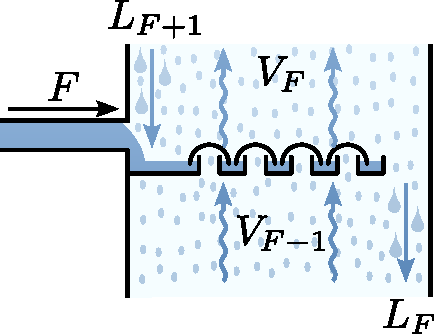
\includegraphics[clip,width=0.5\textwidth]{figures/testfig} 
%\caption{\label{fig:testfig} A test figure.} 
%\end{figure}


% %\section{References} 
%You can reference entries in your bib file using the key you have set 
%for it like so~\cite{Bannerman_2009}. I can even do cool things like 
%say the author of that citation is \citeauthor{Bannerman_2009} and it 
%was published in \citeyear{Bannerman_2009}. Or even ask for a full
%citation, like so: \fullcite{Bannerman_2009}. % 
%But you must remember toprintthe bibliography at the end of every 
%chapter!
\newpage\printbibliography[heading=thesisChapterBib] 

\appendix
\chapter{Derivation of Collision Dynamics for Stepped Potentials }
\label{app:derivation}
Considering a collision between particles $i$ and $j$, each with mass,
$m$ with a step energy difference of $\Delta \Phi$, the conservation of
momentum is shown in equation \eqref{eq:consMom}. Here the prime
indicates post-collision values.

\begin{equation}
\label{eq:consMom}
m\mathbf{v}_i + m\mathbf{v}_j = m\mathbf{v}'_i + m\mathbf{v}'_j
\end{equation}

The momentum change of each particle must occur along the separation
vector between the two particles, which can be expressed by equation
\eqref{eq:defA}, where $A$ is an arbitary coefficient.

\begin{equation}
  \label{eq:defA}
  m\mathbf{v}_i - m\mathbf{v}'_i = -(m\mathbf{v}_j - m\mathbf{v}'_j) 
  = -A\mathbf{\hat{r}}_{ij}
\end{equation}

Energy must also be conserved in the system so equation
\eqref{eq:constE} must also apply.  This can be rewritten to equations
\eqref{eq:constE1} and \eqref{eq:constE2}

\begin{equation}
  \label{eq:constE}
  \frac{1}{2}mv_i^2 + \frac{1}{2}mv_j^2 =
  \frac{1}{2}m{v'_i}^2 + \frac{1}{2}m{v'_j}^2 + \Delta \Phi
\end{equation}

\begin{equation}
  \label{eq:constE1}
  v_i^2 - {v'_i}^2 +
  v_j^2 - {v'_j}^2 - \frac{2}{m}\Delta \Phi = 0
\end{equation}

\begin{equation}
  \label{eq:constE2}
  (\mathbf{v}_i - \mathbf{v}'_i)\cdot(\mathbf{v}_i + \mathbf{v}'_i) +
  (\mathbf{v}_j - \mathbf{v}'_j)\cdot(\mathbf{v}_j + \mathbf{v}'_j) -
  \frac{2}{m}\Delta \Phi = 0
\end{equation}

Equation \eqref{eq:defA} can now be substituted into
\eqref{eq:constE2} to give equation \eqref{eq:eq1}.

\begin{equation}
  \label{eq:eq1}
  \frac{A}{m}\mathbf{\hat{r}}_{ij} (\mathbf{v}_j - \mathbf{v}_i 
  + \mathbf{v}'_j - \mathbf{v}'_i) - \frac{2}{m}\Delta \Phi = 0
\end{equation}

Equation \eqref{eq:defA} and the definition of the separation velocity
vector ($\mathbf{v}_{ij} = \mathbf{v}_i - \mathbf{v}_j$) can be
substituted into equation \eqref{eq:eq1} to give \eqref{eq:eq2}.

\begin{equation}
  \label{eq:eq2}
  -\frac{A^2}{m}
  -A\mathbf{\hat{r}}_{ij}\cdot\mathbf{v}_{ij} - \Delta \Phi = 0
\end{equation}

This is a quadratic equation in terms of $A$ therefore it's roots must
be given by equation \eqref{eq:devQuadratic}.

\begin{equation}
  \label{eq:devQuadratic}
  A = -\frac{m}{2}\left((\mathbf{v}_{ij}\cdot\mathbf{\hat{r}}_{ij}) \pm
  \sqrt{(\mathbf{v}_{ij}\cdot\mathbf{\hat{r}}_{ij})^2 - \frac{4}{m}\Delta \Phi}\right)
\end{equation}  

From equation \eqref{eq:defA}, the change in velocity of each particle
is given in equations \eqref{eq:deltaV}

\begin{subequations}
  \label{eq:deltaV}
  \begin{align}
    \Delta\mathbf{v}_i &= \frac{A}{m} \mathbf{\hat{r}}_{ij} \\
    \Delta\mathbf{v}_j &= -\frac{A}{m}\mathbf{\hat{r}}_{ij}    
  \end{align}
\end{subequations}

\end{document}

%%%%TAYLOR SERIES FOR GEAR'S ALGORITHM%%%% %\begin{equation} 
%\begin{aligned}
%\vec{r}(t+\Delta t) &= \vec{r}(t) + \vec{v}(t) \Delta t 
% +\frac{1}{2}\vec{a}(t)\Delta t^2 + \frac{1}{3!}\vec{b}(t)\Delta t^3 
% +\frac{1}{4!}\vec{c}(t)\Delta t^4 + \frac{1}{5!}\vec{d}(t)\Delta t^5 \\
%\vec{v}(t+\Delta t) &= \vec{v}(t) \Delta t + \vec{a}(t)\Delta t^2 
% +\frac{1}{2}\vec{b}(t)\Delta t^3 + \frac{1}{3!}\vec{c}(t)\Delta t^4 +
%\frac{1}{4!}\vec{d}(t)\Delta t^5 \\ %\vec{a}(t+\Delta t) &= \vec{a}(t)\Delta
%t^2+ \vec{b}(t)\Delta t^3 % + \frac{1}{2!}\vec{c}(t)\Delta t^4 +
%\frac{1}{3!}\vec{d}(t)\Delta t^5 \\ %\vec{b}(t+\Delta t) &= \vec{b}(t)\Delta
%t^3+ \vec{c}(t)\Delta t^4 % + \frac{1}{2!}\vec{d}(t)\Delta t^5 \\
%\vec{c}(t+\Deltat) &= \vec{c}(t)\Delta t^4 + \vec{d}(t)\Delta t^5 \\
%\vec{d}(t+\Delta t) &=
%\vec{d}(t)\Delta t^5 \\ %\end{aligned} %\end{equation}
